%%%%%%%%%%%%%%%%%%%% author.tex %%%%%%%%%%%%%%%%%%%%%%%%%%%%%%%%%%%
%
% sample root file for your "contribution" to a contributed volume
%
% Use this file as a template for your own input.
%
%%%%%%%%%%%%%%%% Springer %%%%%%%%%%%%%%%%%%%%%%%%%%%%%%%%%%


% RECOMMENDED %%%%%%%%%%%%%%%%%%%%%%%%%%%%%%%%%%%%%%%%%%%%%%%%%%%
\documentclass[graybox]{svmult}

% choose options for [] as required from the list
% in the Reference Guide

\usepackage{mathptmx}       % selects Times Roman as basic font
\usepackage{helvet}         % selects Helvetica as sans-serif font
\usepackage{courier}        % selects Courier as typewriter font
\usepackage{type1cm}        % activate if the above 3 fonts are
                            % not available on your system
%
\usepackage{makeidx}         % allows index generation
\usepackage{graphicx}        % standard LaTeX graphics tool
                             % when including figure files
\usepackage{epstopdf}

\usepackage[hang, small,labelfont=bf,up,textfont=it,up]{caption} % Custom captions under/above floats in tables or figures
\usepackage{subcaption}
\captionsetup{compatibility=false} % otherwise it raises some issues regarding compatibility

\usepackage{multicol}        % used for the two-column index
\usepackage[bottom]{footmisc}% places footnotes at page bottom
\usepackage{amsmath}
\usepackage{amssymb}
\usepackage{mathtools}
%\usepackage[linesnumbered, ruled, vlined]{algorithm2e}
%\usepackage{algorithm}% http://ctan.org/pkg/algorithms
%\usepackage{algorithmicx} 
%\usepackage{algpseudocode}% http://ctan.org/pkg/algorithmicx
%\renewcommand{\algorithmicrequire}{\textbf{Input:}}
%\renewcommand{\algorithmicensure}{\textbf{Output:}}
\usepackage{enumerate}
\usepackage{multirow}
\usepackage{cleveref}

\newcommand{\commnet}{\color{red}}

\usepackage{tikz}
\usepackage{pgfplots}
\usepackage{pgfplotstable}
\pgfplotsset{
    % most recent feature set of pgfplots
    compat=newest,
    % some settings for grid
    grid style={black!20!white, thin, densely dotted},
    % modify plot appearance
    every axis plot/.append style={no markers, thick},
    % i like the labels a bit smaller
    label style={font=\small},
    tick label style={font=\small}
}
\usepgfplotslibrary{external} 
\tikzexternalize[prefix=TikzFigures/]

%\usepackage[hang, small,labelfont=bf,up,textfont=it,up]{caption} % Custom captions under/above floats in tables or figures
\usepackage{booktabs} % Horizontal rules in tables
\usepackage{float} % Required for tables and figures in the multi-column environment - they need to be placed in specific locations with the [H] (e.g. \begin{table}[H])
%\usepackage{hyperref} % For hyperlinks in the PDF

% see the list of further useful packages
% in the Reference Guide

\makeindex             % used for the subject index
                       % please use the style svind.ist with
                       % your makeindex program

\pgfplotsset{every tick label/.append style={font=\Large}}

%%%%%%%%%%%%%%%%%%%%%%%%%%%%%%%%%%%%%%%%%%%%%%%%%%%%%%%%%%%%%%%%%%%%%%%%%%%%%%%%%%%%%%%%%

\begin{document}

\title*{Conservative Model Order Reduction for Fluid Flow}
% Use \titlerunning{Short Title} for an abbreviated version of
% your contribution title if the original one is too long
\author{Babak Maboudi Afkham, Nicol\`o Ripamonti, Qian Wang, and Jan S. Hesthaven}
% Use \authorrunning{Short Title} for an abbreviated version of
% your contribution title if the original one is too long
\institute{B. Maboudi Afkham, N. Ripamonti, Q. Wang, J.S. Hesthaven \at EPFL, Lausanne, Switzerland \email{babak.maboudi@epfl.ch}}
%
% Use the package "url.sty" to avoid
% problems with special characters
% used in your e-mail or web address
%
\maketitle

%\abstract*{Each chapter should be preceded by an abstract (10--15 lines long) that summarizes the content. The abstract will appear \textit{online} at \url{www.SpringerLink.com} and be available with unrestricted access. This allows unregistered users to read the abstract as a teaser for the complete chapter. As a general rule the abstracts will not appear in the printed version of your book unless it is the style of your particular book or that of the series to which your book belongs.
%Please use the 'starred' version of the new Springer \texttt{abstract} command for typesetting the text of the online abstracts (cf. source file of this chapter template \texttt{abstract}) and include them with the source files of your manuscript. Use the plain \texttt{abstract} command if the abstract is also to appear in the printed version of the book.}

%\abstract{In the context of model order reduction, conservation of stability for systems of hyperbolic partial differential equations, remains a challenge. Recently preserving structures, invariants and conservation laws, in order to help with stability, and ensure robustness in long-time integrations, has been an area of active research. Energy conservation is a fundamental feature of fluid flows which is often violated in the course of model reduction. In this paper we discuss a model reduction routine, that exploits skew-symmetry of conservative and centered discretization schemes, to recover conservation of energy at the level of reduced system. This results in an, overall, correct evolution of the fluid and ensures robustness of the reduced system. We evaluate the performance of the proposed method through numerical simulation of various fluid flows, and also in a numerical simulation of continuous variable resonance combustor model.}

\abstract{In the past decade, model order reduction (MOR) has been successful in reducing the computational complexity of elliptic and parabolic systems of partial differential equations (PDEs). However, MOR of hyperbolic equations remains a challenge. Symmetries and conservation laws, which are a distinctive feature of such systems, are often destroyed by conventional MOR techniques which result in a perturbed, and often unstable reduced system. The importance of conservation of energy is well-known for a correct numerical integration of fluid flow. In this paper, we discuss model reduction, that exploits skew-symmetry of conservative and centered discretization schemes, to recover conservation of energy at the level of the reduced system. Moreover, we argue that the reduced system, constructed with the new method, can be identified by a reduced energy that mimics the energy of the high-fidelity system. Therefore, the loss in energy, associated with the model reduction, remains constant in time. This results in an, overall, correct evolution of the fluid that ensures robustness of the reduced system. We evaluate the performance of the proposed method through numerical simulation of various fluid flows, and through a numerical simulation of a continuous variable resonance combustor model.}


% sections are added here

\section{Introduction} \label{sec:intro}

Model order reduction (MOR), and in particular reduced basis (RB) methods, has emerged as a powerful approach to cope with the complex and computationally intensive models in engineering and science. Such techniques construct a reduced ordered representation for the state of a model which accurately approximates the configuration of the system. The evaluation of this representation is then possible with considerable acceleration.

Although RB methods are successful in reducing the computational complexity of models with elliptic and parabolic partial differential equations (PDEs), MOR of systems of hyperbolic equations, or models with strong advective terms, remains a challenge. Often, such models arise from a set of invariants and conservation laws, some of which are violated by MOR which result in a qualitatively wrong, and sometimes unstable, solution.

Constructing MOR techniques and RB methods that preserve intrinsic structures has recently attracted attention \cite{doi:10.1137/17M1111991,kalashnikova2014stabilization,farhat2015structure,doi:10.1137/110836742,beattie2011structure,doi:10.1137/140978922}. Structure preservation can recover a physically meaningful reduced model, rather than a pure algebraic coupling of equations. This enforces robustness and can help with the stability of the reduced model. Preserving time-symmetries of Lagrangian, Hamiltonian, and port-Hamiltonian systems can be found in the works of \cite{Carlberg:2014ky,doi:10.1137/140978922,doi:10.1137/17M1111991,beattie2011structure,chaturantabut2016structure,gugercin2012structure}. Conserving inf-sup stability, in the context of finite element methods, can be found in \cite{farhat2015structure,ballarin2015supremizer}. Furthermore, a flux preserving model reduction for finite volume methods is presented in \cite{carlberg2018conservative}. 

Large scale simulations of fluid flows arise in a wide range of disciplines and industries. Therefore, MOR of fluid flows, specially when advective terms are dominant, is important. It is well known that conservation of the energy, specially kinetic energy, is essential for a qualitatively correct numerical integration of fluid flows. Conventional model reduction techniques often violates conservation of mass, momentum \cite{carlberg2018conservative}, or energy in fluid flows which result in an unstable reduced system, in particular for long time-integration. The method discussed in \cite{carlberg2018conservative} conserves the mass and momentum for a finite volume discretization scheme. However, a method that also conserves the energy of the fluid flow is not known to the authors.

Skew-symmetric formulation of fluid flows constructs a skew-symmetric differential operator, acting on the momentum vector field, that ensures conservation of quadratic invariants, such as energy. Combined wirh centered time and space discretization schemes, typically a finite differences discretization method, they recover time-symmetries of a fluid at the discrete level. Such discretization schemes are studies comprehensively over the past few decades and can be found in the works of \cite{morinishi2010skew,morinishi1998fully,desjardins2008high,tadmor1984skew,reiss2014conservative} and the references therein.

In this paper we discuss how to preserve skew-symmetry of the differential operators at the level of the reduced system. This results in conservation of quadratic invariants. Furthermore, we show that the reduced system, as a system of coupled differential equations, contains quadratic invariants and an associated energy which approximates the energy of the high-fidelity system. Therefore, a proper time stepping scheme preserves the reduced representation of the energy, and therefore, the loss in energy due to model reduction remains constant in time. Furthermore, we demonstrate, through numerical experiments, that a quasi-skew-symmetric form of fluid flow, i.e. a formulation where only spacial differential operators are in a skew-symmetric form, offer remarkable stability properties in terms of MOR. This allows an explicit time-integration to be utilized while recovering robustness of skew-symmetric forms at the reduced level.

The rest of this paper is organized as follows. In \Cref{sec:mor} we summarize the theory on MOR and introduce the proper orthogonal decomposition (POD) as a conventional RB method. We discuss skew-symmetric and conservatives methods for compressible and incompressible fluid flows in \Cref{sec:skew}. Conservative and energy-preserving model reduction of fluid flows is discussed in \Cref{sec:mor_skew}. We evaluate the performance of the method through numerical simulations of incompressible and compressible fluid flow in \Cref{sec:res}. We also apply the method to construct a reduced system for the continuous variable resonance combustor, a one dimensional reaction-diffusion model for a rocket engine. Finally, we present conclusive remarks in \Cref{sec:con}.

\section{Model Order Reduction for Time Dependent Problems} \label{sec:mor}

Consider a dynamical system of the form
\begin{equation} \label{eq:1}
	\left\{
	\begin{aligned}
		\frac{d}{dt} u(t) &= f(t,u(t)),\\
		u(0) &= u_0.
	\end{aligned}
	\right.
\end{equation}
Here, $u(t),u_0\in \mathbb R^{n}$ and $f: [0,T]\times \mathbb R^{n} \to \mathbb R^{n}$, for some $T<\infty$, is a Lipschitz function. We may apply the \emph{method of lines} \cite{Edsberg:2008:ICM:1477735} to a system of partial differential equations to obtain a dynamical system of the form \eqref{eq:1}. The \emph{solution manifold} for \eqref{eq:1} is defined as
\begin{equation} \label{eq:2}
	\mathcal M_u := \{ u(t) | t \in [0,T] \}.
\end{equation}
When $\mathcal M_u$ has a low-dimensional representation, it is referred to as \emph{reducible}. Assume that $\mathcal M_u$ can be well approximated by $k$-dimensional linear subspace $\mathcal V_k$, with $k\ll n$ and let $E_k = \{ v_1,\dots,v_k \}$ be the basis vectors for $\mathcal V_k$ and $V_k$ the basis matrix that contains these vectors in its columns. A reduced basis (RB) method assumes that $u \approx \tilde u = V_k v$, where $v$ is the expansion coefficients of $\tilde u$ in the basis $E_k$. Substituting this into \eqref{eq:1} yields
\begin{equation} \label{eq:3}
	V_k \frac{d}{dt} v(t) = f(t,V_{k}v) + r(t,u).	
\end{equation}
Here, $r$ is the error vector in this approximation. The Petrov-Galerkin projection of \eqref{eq:1} onto $\mathcal V_k$ requires $r$ to be orthogonal to a $k$-dimensional subspace $\mathcal W_k$. One can construct a projection operator $P_{\mathcal V_{k},\mathcal W_k}$ that projects elements of $\mathbb R^{n}$ onto $\mathcal V_k$, orthogonal to $\mathcal W_k$ as $P_{\mathcal V_{k},\mathcal W_k} = V_k(W_k^TV_k)^{-1}W_k^T$, where $W_k$ is the basis matrix that contains the basis vectors of $\mathcal W_k$ in its columns and $W_k^TV_k$ is assumed to be invertible. With this projection, \eqref{eq:1} reduces to
\begin{equation} \label{eq:4}
	\left\{
	\begin{aligned}
		\frac{d}{dt} v(t) &= (W_k^TV_k)^{-1} f(t,V_{k}v),\\
		v(0) &= (W_k^TV_k)^{-1}u_0.
	\end{aligned}
	\right.
\end{equation}
When we require $W_k=V_k$, then \eqref{eq:4} is referred to as the \emph{Galerkin} projection of \eqref{eq:1} onto $\mathcal V_k$. Since \eqref{eq:4} has a smaller size, as compared to \eqref{eq:1}, one can expect accelerated evaluation. To numerically identify the best possible subspace $\mathcal V_{k}$ we first discretize the solution manifold to obtain
\begin{equation} \label{eq:5}
	\mathcal M_{u}^{\Delta} = \{ u(t_i) | i\in \{ 1,\dots,N_t \} \}.
\end{equation}
Members of $M_{u}^{\Delta}$ are referred to as \emph{snapshots} of \eqref{eq:1}. One can obtain these snapshots by applying a time-integration scheme, e.g. the Runge-Kutta methods, to \eqref{eq:1} to obtain $\tilde {\mathcal M}_{u}^{\Delta}$ an approximation to $\mathcal M_{u}^{\Delta}$. Throughout this paper, we assume that we can choose $\tilde{\mathcal M}_{u}^{\Delta}$ arbitrary close to $\mathcal M_{u}^{\Delta}$, therefore, by an abuse of notation, we may drop the overscript ``\textasciitilde''. For a Galerkin projection, the best possible basis $V_k$ is the one that minimizes the collective projection error \cite{hesthaven2015certified}, i.e., the solution to the minimization problem
\begin{equation} \label{eq:6}
\begin{aligned}
&  \underset{V_k\in\mathbb R^{n\times k}}{\text{minimize}}
& &  \| S - V_kV_k^TS\|_F, \\
& \text{subject to}
& & V_k^TV_k=I_k.
\end{aligned}
\end{equation}
Here $S$ collects vectors in $\mathcal M_{u}^{\Delta}$ in its columns, referred to as the \emph{snapshot matrix}, $\|\cdot \|_F$ is the Frobenius norm \cite{trefethen97}, and $I_{k}$ is the identity matrix of size $k$. Note that the constraint in \eqref{eq:6} requires $V_k$ to be orthonormal. The basis matrix $V_k$ that solves the minimization problem \eqref{eq:6} is referred to as the \emph{proper orthogonal decomposition} (POD) of $S$ of size $k$ \cite{hesthaven2015certified}, and, according to the Schmidt-Mirsky theorem, can be constructed using the left singular vectors of $S$ as
\begin{equation}
	V_{k} = [u_i]_{i=1}^{k}.
\end{equation}
Here $u_i$, for $i=1,\dots k$, are the first $k$ singular vectors of $S$.

Often MOR is studied in the parametric setting, where the vector $u,u_0$, and the right hand side $f$ of \eqref{eq:1} are of the form $u(t;\mu)$, $u_0(\mu)$, and $f(t,u;\mu)$, respectively. Here $\mu$ belongs to $\mathbb P$ a closed subset of $\mathbb R^d$. In this case, the reduced system can approximate the quantities of interest at an accelerated rate. Since the nature of time, as a parameter, is different from other spacial and physical parameters, in this paper we solely focus on $t$ as the parameter. Nevertheless, it is straight forward to extend the results of this paper to the parameter setting by using POD in time and parameter space, or by using the POD-greedy \cite{haasdonk2013convergence,hesthaven2015certified,quarteroni2015reduced} method to generate a basis $V_k$.

Since the approximated solution $\tilde u$ is a linear combination of the POD basis vectors, $\tilde u$ inherits linear properties of these basis vectors. However, when the solution $u$ to \eqref{eq:1} satisfies some nonlinear invariants, there is no guarantee that, in general, $\tilde u$ also satisfy such invariants \cite{doi:10.1137/140959602,doi:10.1137/140978922,doi:10.1137/17M1111991,MaboudiAfkham2018}. This results in a qualitatively wrong and often unstable solution. In the later sections, we discuss how the skew-symmetric formulation of the fluid flow allows conservation of quadratic invariants, e.g. the kinetic energy, at the level of the reduced system.

\section{Skew Symmetric and Centered Schemes for Fluid Flows} \label{sec:skew}

In this section we summarize the conservation properties of skew-symmetric forms and discretization schemes, following, closely, the works of \cite{morinishi2010skew,morinishi1998fully,tadmor1984skew,reiss2014conservative}.

\subsection{Conservation Laws} \label{sec:skew.1}
In the context of fluid flows, transport of conserved quantities, can be expressed as
\begin{equation} \label{eq:3.1}
	\frac{\partial }{\partial t} \rho \varphi + \nabla \cdot ( \rho u \varphi  ) = \nabla \cdot F_{\varphi}\quad \text{defined in} \quad \Omega \subset \mathbb R^{d}.
\end{equation}
Here, $d = 1,2$ or $3$, $\rho:\Omega\to \mathbb R$ is the density, $u\in \Omega \to \mathbb R^{d}$ is the velocity vector field, $\varphi$ is a measured scalar quantity of the flow, and $F_{\varphi}$ is the flux function associated to $\varphi$. Integration of \eqref{eq:3.1} over $ \Omega$ yields
\begin{equation} \label{eq:3.2}
	\frac{d}{dt} \int_{\Omega} \rho \varphi \ dx = \int_{\partial \Omega} (F_{\varphi} - \rho u \varphi) \cdot \hat n\ ds,
\end{equation}
where $\partial \Omega$ is the boundary of $\Omega$, and $\hat n$ is the unit outward normal vector to $\partial \Omega$. \edit{This means that the quantity $(\rho\varphi)$ is explicitly conserved over control volumes.} Therefore, \eqref{eq:3.1} is referred to as the \emph{conservative form} and the convective term in \eqref{eq:3.1} is referred to as the \emph{divergence form}. However, using the \emph{continuity equation}
\begin{equation} \label{eq:3.3}
	\frac{\partial }{\partial t} \rho + \nabla \cdot (\rho u) = 0,
\end{equation}
we can rewrite \eqref{eq:3.1} as
\begin{equation} \label{eq:3.4}
	\rho \frac{\partial }{\partial t} \varphi + (\rho u)\cdot \nabla \varphi = \nabla \cdot F_{\varphi}.
\end{equation}
The convective term in this formulation is referred to as the \emph{advective form}. The \emph{skew-symmetric} form of the convective term is obtained by the arithmetic average of the divergent and the advective form:
\begin{equation} \label{eq:3.5}
	\frac{1}{2} \left( \rho \frac{\partial }{\partial t} \varphi + \frac{\partial }{\partial t} (\rho \varphi) \right) + \frac 1 2 \left( (\rho u)\cdot \nabla \varphi + \nabla \cdot (\rho u \varphi) \right) = \nabla \cdot F_{\varphi}.
\end{equation}
Multiplying \eqref{eq:3.5} with $\varphi$ yields
\begin{equation}
	\frac{\partial }{\partial t} \rho \varphi^2 + \nabla \cdot ( \rho u \varphi^2  ) = \varphi \nabla \cdot F_{\varphi}.
\end{equation}
\edit{Therefore, $\rho \varphi^2$} is a conserved quantity for a flux-free $\varphi$. Since the divergence, the advective and the skew-symmetric forms are identical at the continuous level, $\varphi^2$ is a conserved quantity for all forms. However, the equivalence of these forms is not preserved through a general discretization scheme and we can not expect $\varphi^2$ to be a conserved quantity at the discrete level. To motivate numerical advantages of the skew-symmetric form consider the operator 
\begin{equation}
	S_{\rho u}(\cdot) = \frac 1 2 ( [ \nabla \cdot \rho u ] + (\rho u)\cdot \nabla )(\cdot).
\end{equation}
With a proper set of boundary condition, this operator is a skew-adjoint operator on $L^2$. Here, $[\cdot]$ indicates that the inside of the brackets act as a differential operator. This skew-adjoint property is used later to show the conservation of some quadratic quantities in \eqref{eq:3.1}. Similarly, we can define a skew-adjoint operator with respect to the time variable as
\begin{equation}
	S_{\rho,\partial_t} = \frac{1}{2} \left( \rho \frac{\partial}{\partial t} + [ \frac{\partial}{\partial t} \rho] \right).
\end{equation}
Here, the subscript $\partial t$ is to emphasize that $S_{\rho,\partial_t}$ is a differential operator with respect to $t$. A proper time and space discretization of $S_{\rho u}$ and $S_{\rho,\partial_t}$ can preserve the skewness property.

Numerical time integration of \eqref{eq:3.5} can be challenging since the time differentiation of different variables is present. Following \cite{morinishi2010skew}, we rewrite \eqref{eq:3.5} as
\begin{equation} \label{eq:3.6}
	\sqrt{\rho } \frac{\partial }{\partial t} (\sqrt \rho \varphi ) + S_{\rho u}(\varphi) = \nabla \cdot F_{\varphi}.
\end{equation}
Time integration of this form is presented in \cite{morinishi2010skew,reiss2014conservative}. Note that one can also generate a quasi-skew-symmetric form \cite{blaisdell1991numerical,morinishi2003dns} of \eqref{eq:3.1} as
\begin{equation} \label{eq:3.7}
	\frac{\partial }{\partial t} (\rho \varphi) + \edit{ \frac 1 2 \left( \nabla \cdot(\rho u \varphi) + \rho u \cdot \nabla \varphi + \varphi \nabla \cdot(\rho u) \right) } = \nabla \cdot F_{\varphi}.
\end{equation}
Even though this is not a fully skew-symmetric form (skew-symmetric only in space), the numerical stability of this form is significantly better than the divergence and advective form \cite{morinishi2010skew,blaisdell1991numerical,morinishi2003dns}. Note that this quasi-skew-symmetric form is identical to the skew-symmetric form in the incompressible limit.

\subsection{Incompressible Fluid} \label{sec:skew.2}
Consider the governing equations of an incompressible fluid with skew-symmetric convective term:
\begin{equation} \label{eq:3.8}
	\left\{
	\begin{aligned}
	&\nabla \cdot u = 0, \\
	&\frac{\partial}{\partial t} u + S_{u}(u) + \nabla p = \nabla \cdot \tau,
	\end{aligned}
	\right.
\end{equation}
defined on $\Omega$. Here, $p: \Omega \to \mathbb R^+$ is the pressure, $\tau: \Omega \to \mathbb R^{d\times d}$ is the viscous stress tensor, and $S_u = \frac 1 2 ([ \nabla \cdot u] + u\cdot \nabla)$. It is straight forward to check
\begin{equation} \label{eq:3.9}
	\frac{d}{dt} K + \nabla \cdot (Ku) + \nabla \cdot (pu)= \nabla \cdot (\tau u) - (\tau \nabla)\cdot u,
\end{equation}
where $K = \frac 1 2 \sum_{i=1}^d u_i^2 $ is the kinetic energy and we used 
\begin{equation} \label{eq:3.11}
	u\cdot S_{u}(u) = \nabla \cdot(Ku).
\end{equation}
The only non-conservative term in \eqref{eq:3.9} is $-(\tau \nabla)\cdot u$, which corresponds to dissipation of kinetic energy. Therefore, in the absence of the viscous terms, $K$ is a conserved quantity of the system, and $\frac d {dt} \int_{\Omega} K \ dx <0$ when $\tau\neq 0$. Note that as long as $\nabla \cdot u = 0$, as discussed in \Cref{sec:skew.1}, the divergence, the convective, and the skew-symmetric forms are identical for the incompressible fluid equation. Thus, kinetic energy is conserved for all forms. However, for a general discretization scheme, these forms are not identical and often conservation of kinetic energy (in the discrete sense) may be violated.

A skew-symmetric discretization of \eqref{eq:3.8} is a centered scheme that exploits the skew-adjoint property of $S_u$, and ensures conservation of kinetic energy at the discrete level. We uniformly discretize $\Omega$ into $N$ points and denote by $\mathbf u \in \mathbb R^{N\times d}$, $\mathbf p \in \mathbb R^N$, and $T \in R^{N\times d\times d} $ the discrete representation of $u$, $p$, and $\tau$, respectively. Let $D_j$ be the centered finite difference scheme for $\partial / \partial x_j$, and for $j = 1,\dots,d$. The momentum equation in \eqref{eq:3.8} is discretized as
\begin{equation} \label{eq:3.13}
	\frac{d}{dt}{\mathbf u}_i + S_{\mathbf u} \mathbf u_i + D_i \mathbf p = \sum_{j=1}^d D_j T_{ij}, \quad i=1,\dots,d,
\end{equation}
where $S_{\mathbf u}$ is the discretization of $S_{u}$ given by
\begin{equation} \label{eq:3.14}
	S_{\mathbf u} = \sum_{j=1}^d D_j U_j + U_j D_j,
\end{equation}
and $U_i$ contains components of $\mathbf u_i$ on its diagonal. We require $D_i$ to satisfy
\begin{enumerate}
	\item $D_i = -D_i^T$
	\item $D_i \mathbf 1 = \mathbf 0$, where $\mathbf 1$ and $\mathbf 0$ are vectors of ones and zeros, respectively.
\end{enumerate}
Conditions 1 and 2 yield
\begin{equation} \label{eq:3.15}
	S_{\mathbf u} = -S_{\mathbf u}^T, \quad \mathbf 1^T S_{\mathbf u} \mathbf u_i = 0, \quad i=1,\dots,d.
\end{equation}
Conservation of momentum in the discrete sense is expressed as
\begin{equation} \label{eq:3.16}
	\frac{d}{dt} \sum_{i=1}^d  \mathbf 1^T \mathbf u_i = \sum_{i=1}^d \left( - \mathbf 1^T S_{\mathbf u} \mathbf u_i - \mathbf 1^T D_i \mathbf p + \sum_{j=1}^d \mathbf 1^T D_j T_{ij}  \right) = 0.
\end{equation}
Similarly, it is verified that
\begin{equation} \label{eq:3.17}
\frac{d}{dt} \sum_{i=1}^d \left( \frac 1 2 \mathbf u_i^T \mathbf u_i \right) = - \sum_{i,j=1}^d T_{ij}D_j \mathbf u_i \leq 0.
\end{equation}
Conditions 1 and 2 for $D_i$ are easily checked for a centered finite differences scheme on a periodic domain. For other types of boundaries, e.g., wall boundary and inflow/outflow, we refer the reader to \cite{morinishi1998fully,desjardins2008high} for the construction of the proper discrete centered differentiation operator. We note that the finite differences schemes are chosen here for illustration purposes. It is easily checked that any discrete differentiation operator that satisfies discrete integration by parts, e.g. summation by part (SBP) methods and discontinuous Galerkin (DG) methods, also satisfies conditions 1 and 2 and can be used to construct a skew-symmetric discretization.

\subsection{Compressible Fluid} \label{sec:skew.3}
Consider the equations governing the evolution of a compressible fluid in a skew-symmetric form in one spacial dimension
\begin{equation} \label{eq:3.18}
\left\{
\begin{aligned}
	&\frac{\partial}{\partial t} \rho + \frac{\partial }{\partial x}(\rho u) = 0, \\ 
	& S_{\rho,\partial_t}(u)+ S_{\rho u}(u) + \frac{\partial }{\partial x} p = \frac{\partial }{\partial x} \tau, \\
	&\frac{\partial}{\partial t} \rho E + \frac{\partial}{\partial x}(u E + up) = \frac{\partial }{\partial x}(u\tau - \phi).
\end{aligned}
\right.
\end{equation}
Here $E= e + u^2/2$ is the total energy per unit mass, with $e = {p}/{\rho(\gamma - 1)}$ being the internal energy, $\gamma$ the adiabatic gas index, and $\phi = -\lambda \frac{\partial T}{\partial x}$ is the heat flux, with $\lambda$ as the heat conductivity. The remaining variables are the same as those discussed in \Cref{sec:skew.2}. Following \cite{reiss2014conservative}, the evolution of the momentum equation is
\begin{equation} \label{eq:3.19}
	\begin{aligned}
	\frac{\partial}{\partial t}(\frac{\rho u^2}{2}) + \frac{\partial }{\partial x}(\rho u \frac{u^2}{2}) &= \frac 1 2 u( \frac{d}{dt} \rho u + \rho \frac{d}{dt} u ) + \frac 1 2 u ( [ \frac{\partial}{\partial x} \rho u ] u + \rho u \frac{\partial }{\partial x} u ) \\
	& = - u \frac{\partial}{\partial x} p + u \frac{\partial}{\partial x} \tau.
	\end{aligned}
\end{equation}
Substituting this into the energy equation in \eqref{eq:3.18}, while assuming a constant adiabatic index, yields
\begin{equation} \label{eq:3.20}
	\frac{1}{\gamma -1} \frac{d}{dt} p + \frac{\gamma}{\gamma -1} \frac{\partial }{\partial x} up - u \frac{\partial }{\partial x}(p) = - u \frac{\partial}{\partial x} \tau + \frac{\partial }{\partial x}(u\tau - \phi).
\end{equation}
We discretize the real line, uniformly, into $N$ grid points and denote by $\mathbf r, \mathbf u, \mathbf p \in \mathbb R^{N}$, the discrete representations of $\rho$, $u$, and $p$, respectively. Using the matrix differentiation operator $D\in \mathbb R^{N\times N}$ (we omit the subscript ``$i$'' for the one dimensional case), introduced in \Cref{sec:skew.2}, we define the skew-symmetric matrix operator $S_{\mathbf r \mathbf u} = \frac 1 2 (DUR + RUD)$, where $R$ is the matrix that contains $r$ in its diagonal. Semi-discrete expression of \eqref{eq:3.18} and \eqref{eq:3.20} takes the form
\begin{equation} \label{eq:3.21}
\left\{
\begin{aligned}
	& \frac{d}{dt} \mathbf r + DU\mathbf r = 0, \\
	& S_{\mathbf r,\partial_t} (\mathbf u) + S_{\mathbf r \mathbf u} \mathbf u + D \mathbf p = D T, \\
	&\frac{1}{\gamma -1} \frac{d}{dt} \mathbf p + \frac{\gamma}{\gamma -1} D U \mathbf p - UD\mathbf p = - UDT + D(UT - \mathbf \phi).
\end{aligned}
\right.
\end{equation}
Recalling conditions 1 and 2 for $D$, discussed in \Cref{sec:skew.2}, it is easily verified that
\begin{equation} \label{eq:3.22}
	S_{\mathbf r \mathbf u}^T = - S_{\mathbf r \mathbf u}, \quad \mathbf 1^T S_{\mathbf r \mathbf u} \mathbf u = - \mathbf u^T DU \mathbf r.
\end{equation}
Conservation of mass is expressed as
\begin{equation} \label{eq:3.23}
	\frac{d}{dt} (\mathbf 1^T \mathbf r) = - \mathbf 1^T DR\mathbf u = 0. 
\end{equation}
Furthermore, we recover conservation of momentum in the discrete sense as
\begin{equation} \label{eq:3.24}
\begin{aligned}
	\frac{d}{dt}(\mathbf r^T \mathbf u) &= \frac{1}{2} \frac{d}{dt}(\mathbf r^T \mathbf u) + \frac{1}{2} \left( \mathbf r^T \frac d{dt} \mathbf u +\mathbf u^T \frac{d}{dt} \mathbf r \right)\\
	&= \frac{1}{2}u^T \frac d{dt} \mathbf r + \mathbf 1^T S_{\mathbf r,\partial_t} (\mathbf u) \\
	&= -\frac 1 2 \mathbf u^T DU \mathbf r  - \frac 1 2 \mathbf 1^T S_{\mathbf r \mathbf u} \mathbf u - \mathbf 1^T D\mathbf p +  \mathbf 1^T D T = 0.
\end{aligned}
\end{equation}
Here we used \eqref{eq:3.22} and the mass and the momentum equation in \eqref{eq:3.21}. Similarly, for conservation of the total energy, we have
\begin{equation} \label{eq:3.25}
\begin{aligned}
	\frac{d}{dt} \left( \frac{1}{\gamma - 1} \mathbf 1^T \mathbf p + \frac 1 2 \mathbf (R\mathbf u)^T \mathbf u  \right) &= \frac{d}{dt} \left( \frac{1}{\gamma - 1} \mathbf 1^T \mathbf p \right) + \frac 1 2 \mathbf u^T  S_{\mathbf r,\partial_t} (\mathbf u) = 0.
\end{aligned}
\end{equation}
In addition to the conservation of the total energy, the skew-symmetric form of \eqref{eq:3.21} also conserves the evolutions of the kinetic energy:
\begin{equation} \label{eq:3.26}
\begin{aligned}
	\frac{d}{dt} ( \frac 1 2 \mathbf u^T R\mathbf u) = \frac 1 2 \mathbf u^T S_{\mathbf r,\partial_t} (\mathbf u) &= -\mathbf u ^T S_{\mathbf r \mathbf u} \mathbf u + \mathbf u^T D p + \mathbf u^T DT \\
	&= \mathbf u^T D p + \mathbf u^T DT.
\end{aligned}
\end{equation}
Here, we used the skew-symmetry of $S_{\mathbf r \mathbf u}$. Therefore, only the pressure and the viscous terms contribute to a change in the kinetic energy.

We point out that there are other methods to obtain a skew-symmetric form for \eqref{eq:3.18}, that result in the conservation of other quantities. An entropy preserving skew-symmetric form can be found in \cite{sjogreen2010skew}. Furthermore, a fully quasi-skew-symmetric form for \eqref{eq:3.18}, where all quadratic fluxes are in a skew-symmetric form, is shown to minimize aliasing errors \cite{honein2004higher,honein2005numerical}

\subsection{Time integration}
Following \cite{reiss2014conservative,morinishi2010skew} we can construct a fully discrete second order accurate scheme for \eqref{sec:skew.3} as
\begin{equation} \label{eq:3.27}
	\left\{
	\begin{aligned}
	&\frac 1 2 \sqrt{\mathbf r} ^{n+1/2} \frac{\sqrt{\mathbf r}^{n+1} - \sqrt{\mathbf r}^{n}}{\Delta t} + DU^{n+1/2} \mathbf r^{n} = 0, \\
	& \sqrt{\mathbf r} ^{n+1/2}  \frac{\sqrt{ \mathbf R}^{n+1} \mathbf u^{n+1} - \sqrt{\mathbf R}^{n}\mathbf u^n}{\Delta t} + S_{\mathbf r^{n} \mathbf u^n} \mathbf u^{n+1/2}_\alpha + D \mathbf p^{n} = DT^{n}, \\
	& \frac 1 {\gamma -1} \frac{\mathbf p^{n+1} - \mathbf p^n}{\Delta t} + \frac{\gamma}{\gamma -1} D U^{n} \mathbf p^n - U^{n} D \mathbf p^n = - U^{n}D T^{n} + D (U^nT^n - \phi^n),
	\end{aligned}
	\right.
\end{equation}
\edit{and all the variables are stored at the same location with the same resolution (colocated).} Here, \edit{$\mathbf R$ contains elements of $\mathbf r$ on its diagonal,} $\Delta t$ is the time step, superscript $n$ denotes evaluating at $t = n\Delta t$, superscript $n+1/2$ denotes the arithmetic average of a variable evaluated at $t=n\Delta t$ and $t=(n+1)\Delta t$, the square root sign denotes element-wise application of square root, and 
\begin{equation}
	\mathbf u_{\alpha}^{n+1/2} = \frac{\sqrt{\mathbf R}^{n+1} \mathbf u^{n+1} + \sqrt{\mathbf R}^{n} \mathbf u^{n}}{2\sqrt{\mathbf r}^{n+1/2} }.
\end{equation}
As discussed in \cite{reiss2014conservative}, this time discretization scheme preserves the symmetries expressed in \eqref{eq:3.17}, \eqref{eq:3.24}, \eqref{eq:3.25}, and \eqref{eq:3.26}. In the incompressible case, the method reduces to the implicit mid-point scheme \cite{hairer2006geometric}. For further information see \cite{reiss2014conservative,morinishi2010skew}.


\section{Model Reduction of Fluid Flow} \label{sec:mor_skew}
Straight forward model reduction of \eqref{eq:3.8} and \eqref{eq:3.18} does not, in general, preserves symmetries and conservation laws that were presented in \Cref{sec:skew}. In this section we discuss how to exploit the discrete skew-symmetric structure of \eqref{eq:3.13} and \eqref{eq:3.21} to recover conservation of mass, momentum, and energy at the level of reduced system.

Let $V_{\mathbf r}$, $V_{\mathbf r \mathbf u}$, and $V_{\mathbf u_i}$ be the reduced bases for the snapshots of $\mathbf r$, $R \mathbf u$, and $\mathbf u_i$, respectively. For the one dimensional case, the subscript ``$i$'' is omitted and in case of an incompressible fluid, $V_{ \mathbf r}$ and $V_{\mathbf r \mathbf u}$ are not computed. For the purpose of simplicity, we assume that all bases have the size $k$. We seek to project $S_{\mathbf u}$ and $S_{\mathbf r \mathbf u}$ onto the reduced space, such that the projection preserves the skew-symmetry property. The projected operators, using a Galerkin projection, read
\begin{equation} \label{eq:4.1}
	S^r _{\mathbf u} = V_{ \mathbf u_i}^T S _{\mathbf u} V_{ \mathbf u_i}, \quad i=1,\dots,d,
\end{equation}
and
\begin{equation} \label{eq:4.2}
	S^r_{\mathbf r ,\partial_t} =V_{\mathbf r \mathbf u}^T  S_{\mathbf r ,\partial_t} V_{\mathbf u}, \quad S^r _{\mathbf r \mathbf u} = V_{\mathbf r \mathbf u}^T  S _{\mathbf r \mathbf u} V_{\mathbf u}.
\end{equation}
Note that $S^r_{\mathbf r ,\partial_t}$ is not computed explicitly. It is seen that the $S^r _{\mathbf u}$ is already in a skew-symmetric form. On the other hand, $S^r_{\mathbf r ,\partial_t}$ and $S^r _{\mathbf r \mathbf u}$ are not, in general, skew-adjoint and skew-symmetric, respectively. This can be ensured, however, by requiring $V_{\mathbf r \mathbf u} = V_{\mathbf u}$. We denote such a basis by $V_{\mathbf r \mathbf u, \mathbf u}$.Using \eqref{eq:4.1} and \eqref{eq:4.2}, a Galerkin projection of momentum equation in \eqref{eq:3.13} and governing equations for a compressible fluid in \eqref{eq:3.21} take the form
\begin{equation} \label{eq:4.3}
	\frac{d}{dt} {\mathbf u^r}_i + S^r_{\mathbf u} \mathbf u^r_i + V_{\mathbf u_i} ^T D_i \mathbf p = \sum_{j=1}^d V_{k_3, \mathbf u_i}^T D_j T_{ij}(V_{ \mathbf u_i} \mathbf u^r_i), \quad i=1,\dots,d,
\end{equation}
and
\begin{equation} \label{eq:4.4}
\left\{
\begin{aligned}
	& \frac{d}{dt} \mathbf r^r + \sum_{i=1}^k V^T_{\mathbf r}DU_iV_{\mathbf r}\mathbf r^r = 0, \\
	& S^r_{\mathbf r ,\partial_t} + S^r _{\mathbf r \mathbf u} \mathbf u^r + V_{\mathbf r \mathbf u, \mathbf u}^T D \mathbf V_{\mathbf p} \mathbf p^r = V_{\mathbf r \mathbf u, \mathbf u}^T D T, \\
	&\frac{1}{\gamma -1} \frac{d}{dt} \mathbf p^r + \frac{\gamma}{\gamma -1} \mathbf V_{\mathbf p}^T D U V_{\mathbf p} \mathbf p^r - \mathbf V_{\mathbf p}^T UD V_{\mathbf p} \mathbf p^r = - V_{\mathbf p}^T UDT + V_{\mathbf p}^T D(UT - \mathbf \phi).
\end{aligned}
\right.
\end{equation}
Note that in \eqref{eq:4.4}, dependency of $T$ on $V_{\mathbf r \mathbf u , \mathbf u}$ is not shown for abbreviation. In \eqref{eq:4.3} and \eqref{eq:4.4}, $D_i$ is always multiplied from left with a basis matrix or a diagonal matrix. Therefore, the telescoping sum discussed in condition 2 in \Cref{sec:skew.1} cannot be used to show conservation of mass and momentum. However, POD preserves linear properties of snapshots. To demonstrate, let the overscript ``\textasciitilde'' denote the representation of a reduced variable in the high fidelity space. A reduced variable, e.g. density, can be represented as a linear combination of some snapshots as $\mathbf r \approx \tilde{\mathbf r} = \sum_{i=1}^k c_i \mathbf r_i$, for some snapshots $\mathbf r_i$ and some coefficients $c_i \in \mathbb R$, for $i=1,\dots,k$. The conservation of mass, evaluated by $\tilde{\mathbf r}$, reads
\begin{equation} \label{eq:4.5}
	\frac{d}{dt} \mathbf 1^T \tilde {\mathbf r} = \sum_{i=1}^k c_i  \left( \mathbf 1^T \frac{d}{dt} \mathbf r_i \right) = - \sum_{i=1}^k c_i  \left( \mathbf 1^T DR_i\mathbf u_i \right) = 0.
\end{equation}
Here we used the fact that $\mathbf 1^T D = \mathbf 0^T$. Similarly, we recover conservation of momentum
\begin{equation} \label{eq:4.6}
\begin{aligned}
	\frac{d}{dt}(\tilde {\mathbf r}^T \tilde{\mathbf u}) &= \frac{1}{2} \frac{d}{dt}(\tilde{\mathbf r}^T \tilde{\mathbf u}) + \frac{1}{2} \left( \tilde{ \mathbf r }^T \frac d{dt} \tilde{ \mathbf u } + \tilde {\mathbf u}^T \frac{d}{dt} \tilde {\mathbf r} \right)\\
	&= \sum_{i,j=1}^k d_i c_j \left( \mathbf u_i^T \frac{d}{dt} \mathbf r_j + \left( \mathbf r_j^T \frac d{dt} \mathbf u_i +\mathbf u_i^T \frac{d}{dt} \mathbf r_j \right)\right) = 0.\\
\end{aligned}
\end{equation}
Here, $\tilde{\mathbf u} = \sum_{i=1}^k d_i \mathbf u_i$, for some snapshot $\mathbf u_i$ and coefficients $d_i \in \mathbb R$. Denoting by $\{ R \mathbf u\}^r$ the reduced representation of $R\mathbf u$ in basis $V_{\mathbf r \mathbf u , \mathbf u}$, the evolution of kinetic energy reads
\begin{equation} \label{eq:4.7}
	\begin{aligned}
	\frac{d}{dt}\left( \frac 1 2 \tilde{\mathbf u}^T \tilde{ R } \tilde {\mathbf u} \right) &= \frac{d}{dt}\left( \frac 1 2 {\mathbf u^r}^T V_{\mathbf r \mathbf u , \mathbf u}^T V_{\mathbf r \mathbf u , \mathbf u} \{ R \mathbf u\}^r \right) = \frac{d}{dt}\left( \frac 1 2 {\mathbf u^r}^T \{ R \mathbf u\}^r \right) \\
	&= \frac 1 2 \left( {\mathbf u^r}^T \frac{d}{dt} \{ R \mathbf u \}^r + \{ R \mathbf u \}^r \frac{d}{dt} \mathbf u^r \right) \\
	&= \frac 1 2 \left( {\mathbf u^r}^T V_{\mathbf r \mathbf u , \mathbf u}^T V_{\mathbf r \mathbf u , \mathbf u} \frac{d}{dt} \{ R \mathbf u \}^r + \{ R \mathbf u \}^r \frac{d}{dt} V_{\mathbf r \mathbf u , \mathbf u}^T V_{\mathbf r \mathbf u , \mathbf u} \mathbf u^r \right) \\
	&= {\mathbf u^r}^T S^r_{\mathbf r, \partial_t} \mathbf u^r = { \mathbf u^r }^T V_{\mathbf r \mathbf u , \mathbf u} D V_{\mathbf p} \mathbf P^r + { \mathbf u^r }^T V_{\mathbf r \mathbf u , \mathbf u}^T D T.
	\end{aligned}
\end{equation}
In the missing steps in the last line, the skew-symmetry of $S_{\mathbf r \mathbf u}^r$ is used. Note, that only the reduced pressure and the viscous term contribute to the evolution of kinetic energy. Furthermore, the quantity $ \frac 1 2 {\mathbf u^r}^T \{ R \mathbf u\}^r$ is the kinetic energy associated with the reduced system \eqref{eq:4.4} that approximates the kinetic energy of the high-fidelity system \eqref{eq:3.21} and is a quadratic form with respect to the reduced variables. Conservation of kinetic energy for \eqref{eq:4.3} follows similarly. With what discussed above, it is  straight forward to check that
\begin{equation} \label{eq:4.8}
	\frac{d}{dt} \left( \frac{1}{\gamma - 1} \mathbf 1^T \tilde{\mathbf p} + \frac{1}{2} \tilde{\mathbf u}^T \tilde R \tilde{\mathbf u} \right) = 0,
\end{equation}
i.e., the total energy is conserved. We can immediately recognize that $ \mathbf p^r /(\gamma - 1)$ is the internal energy of the reduced system. However, the total internal energy of \eqref{eq:4.4} is a weighted sum, $ b^T\mathbf p^r /(\gamma - 1)$, with $b = V_{\mathbf p}^T \mathbf 1$ which is an approximation of the total internal energy in \eqref{eq:3.21}. From \eqref{eq:4.5}, \eqref{eq:4.6}, \eqref{eq:4.7}, and \eqref{eq:4.8} we conclude the following proposition.
\begin{proposition}
	The loss in the mass, momentum and energy associated with model reduction in \eqref{eq:4.4} is constant in time, and therefore, bounded.
\end{proposition}

\subsection{Assembling Nonlinear Terms and Time Integration}
Nonlinear terms that appear in \eqref{eq:4.3} and \eqref{eq:4.4} are of quadratic nature. These terms can be evaluated exactly using a set of precomputed matrices as proposed in \cite{Benner2018}. As an example, consider
\begin{equation}
	S_{\mathbf u}^r = V^T_{\mathbf u} ( DU + UD ) V^T_{\mathbf u},
\end{equation}
for simplicity in one spacial dimension. We write $U$ as a linear combination of matrices as $U = \sum_{j=1}^k \mathbf u ^r_j U_j$, where $\mathbf u ^r_j$ is the $j$th component of $\mathbf u ^r$, and $U_j$ contains the $j$th column of $V_{\mathbf u}$ on its diagonal. It follows
\begin{equation}
	S_{\mathbf u}^r = \sum_{j=1}^k \mathbf u ^r_j \left( V^T_{\mathbf u} ( DU_j + U_jD ) V^T_{\mathbf u} \right),
\end{equation}
and the matrices $V^T_{\mathbf u} ( DU_j + U_jD ) V^T_{\mathbf u}$ can be computed prior to the time integration of the reduced system. However, the form of the fully discrete system in \eqref{eq:3.27} introduces cubic and even quartic terms. Although, in principle, the same method can be applied to assemble the nonlinear terms, however, the number of precomputed matrices can grow proportional to the order of nonlinear term. 

To accelerate the assembly of the nonlinear terms that require a large number of precomputed matrices, we may approximately evaluate them using the discrete empirical interpolation method (DEIM). This approximation can affect the accuracy of conserved quantities in \eqref{eq:4.4}. Therefore, the accuracy of DEIM approximation should be chosen considerably higher than the one from POD.

To integrate \eqref{eq:4.4} in time, the fully discrete system \eqref{eq:3.27} is modified prior to model reduction, by dividing the mass and momentum equation with $\sqrt{\mathbf r}^{n+1}$. Note that since the new form is identical to \eqref{eq:3.27}, it does not affect the conserved quantities. Subsequently, a basis for $\sqrt{\mathbf r}$, denoted by $V_{\sqrt{\mathbf r}}$, is constructed. The nonlinear terms, are evaluated exactly using the quadratic expansion or approximated using the DEIM.

\section{Numerical Experiments} \label{sec:res}

\subsection{Vortex Merging} \label{sec:res.1}
Consider the 2-dimensional incompressible Euler equation \eqref{eq:3.8} on a square domain $\Omega = [0,2\pi]^2$, with periodic boundary conditions. Spatial derivatives are discretized using a Fourier spectral method. To capture the fine details characterizing the solution, $256\times 256$ modes is used. We consider the evolution of three vortices, with the initial structure given by
\begin{equation}\label{eqn:initial_cond_vort}
\omega = \omega_0 + \sum_{i=1}^{3} \alpha_i e^{-\dfrac{\left(x-x_i\right)^{2}+\left(y-y_i\right)^{2}}{\beta^2}}.
\end{equation}
Here, $\omega = \nabla \times u$ is the vorticity, $(x,y)$ represents the spatial coordinates, $\left( x_i, y_i\right)$ is the center of the $i$th vortex, $\alpha_i$ its maximum amplitude, and $\beta$ controls the effective radius of the vortex. In this example, the center of three vortices are 
\begin{equation}
\left( x_1, y_1 \right) = \left(0.75\pi,\pi\right) , \left( x_2, y_2 \right) = \left(1.25\pi,\pi\right), \left( x_3, y_3 \right) = \left(1.25\pi,1.5\pi\right),
\end{equation}
close to the center of the domain. Two of the vortices have a positive spin with $\alpha_1 = \alpha_2 = \pi$ and the third rotates in the opposite direction with $\alpha_3 = -0.5\pi$. The effective radius of all the vortices is set to $\beta = 1 / \pi$. This arrangement of vortices is an interesting initial condition to study the process of vortex merging. This phenomenon is often a result of fast-moving dipoles of vortices with the same spin facing another vortex \cite{filaments_vort2} of opposite spin. The merging process transfers the vorticity from the initial configuration into long, narrow, and spiral-shaped strips of intense vorticity \cite{filaments_vort}. The formation of such thin vorticity filaments in the fluid may pose numerical challenges, due to aliasing. 

In the context of MOR, conservation of energy and stability is crucial to capturing fine structures. With the absence of natural dissipation, straight forward application of MOR techniques for the Euler equation is often unstable.

To define the initial conditions in terms of the velocity components $u$ and the pressure $p$, we define a stream-function $\Psi$, the solution to the equation 
\begin{equation} \label{eq:5.1}
	- \Delta \Psi = \omega.
\end{equation}
The initial velocity is then given by $\nabla \times \Psi$. To solve the stream-function problem \eqref{eq:5.1}, we require $\int_{\Omega} \omega \ dx= 0$. It is easily verified that this requirement implies $\omega_0 = 0.038$. The pressure is recovered by solving the related Poisson pressure equation 
\begin{equation*}
\Delta p = - \nabla \cdot S_{u}(u),
\end{equation*}
obtained by applying the divergence operator to \eqref{eq:3.8} and using the incompressibility condition.
 The implicit midpoint scheme, to mimic the time integration scheme presented in \eqref{eq:3.27}, is used to integrate in time. The merging phenomenon is simulated for a total of $18$ time units using a temporal step $\Delta t=0.004$.

\Cref{compare_different_models} illustrates the evolution of the kinetic energy for the advective, divergence, and the skew-symmetric form of the high-fidelity system. It is observed that only the skew-symmetric form preserves the kinetic energy, confirming the discussion in \Cref{sec:skew.2}.

%%%%%%%%%%%%%%%%%%%%%%%%%%%%%%%%%%%%%%%%%
%%%%% Comparison Skew symmetric, divergence and advective form %%%%%
%%%%%%%%%%%%%%%%%%%%%%%%%%%%%%%%%%%%%%%%%
\begin{figure}[t]
  \centering
  \begin{subfigure}[]{0.47\linewidth}
  \begin{tikzpicture}[scale=0.58]
    \begin{axis}[ylabel=$K$,
                 xlabel=$t$,
                 label style={font=\Large},
                 legend pos=south west,
                 legend entries={Skew Symmetric form, Divergence form, Advective form},
                 legend style={font=\large},
                 width=1.4\linewidth, 
                 height=1\linewidth,
                 minor x tick num=1,
                 minor y tick num=2,	
                 yticklabel style={/pgf/number format/.cd,fixed,precision=4},
                 scaled x ticks = true,
                 enlargelimits=false,
                 scale only axis]
                 \addplot[color=red,style=solid,style=ultra thick]  table[x = time, y = energy] {./data/Incompressible_Euler/Energy_compare_formulations/energy_skew_symmetric.txt};
                 \addplot[color=blue,style=solid,style=ultra thick]  table[x = time, y = energy] {./data/Incompressible_Euler/Energy_compare_formulations/energy_divergence.txt};
                 \addplot[color=black!50!green,style=solid,style=ultra thick]  table[x = time, y = energy] {./data/Incompressible_Euler/Energy_compare_formulations/energy_convective.txt};
    \end{axis}%  
  \end{tikzpicture}
\caption{}
\label{compare_different_models}
\end{subfigure}
  \begin{subfigure}[]{0.47\linewidth}
\begin{tikzpicture}[scale=0.58]
    \begin{semilogyaxis}[ylabel = $\frac{\sigma_j}{\sum_i \sigma_i}$,
                 xlabel=Basis POD,
                 label style={font=\Large},
                 %legend pos=north east,
                 %legend entries={$k=24$ Div,$k=102$ Div,$k=201$ Div,$k=24$ Skew,$k=102$ Skew,$k=201$ Skew},
                 legend style={font=\large},
                 grid=both,
                 ticks=both,
                 width=1.4\linewidth, 
                 height=1\linewidth,
                 minor x tick num=1,
                 minor y tick num=2,	
                 yticklabel style={/pgf/number format/.cd,fixed,precision=9},
                 scaled x ticks = true,
                 enlargelimits=false,
                 scale only axis,
                 ymin=0,
                 ymax = 2,
                 samples = 100]
                 \addplot[color=black,style=solid,style=ultra thick]  table[x = x, y = s] {./data/Incompressible_Euler/Singular_values/sv.txt};
    \end{semilogyaxis}
\end{tikzpicture}
\caption{}
\label{singular_values_decay}
\end{subfigure}
  \caption{(\protect\subref{compare_different_models}) The kinetic energy $K$ for the advective, divergence and the skew-symmetric formulations. (\protect\subref{singular_values_decay}) The decay of the singular values for the vortex merging. }
  \label{fig:unstable_full_models}
\end{figure}
A total of $5000$ temporal snapshots is used to construct a reduced basis, following the process discussed in \Cref{sec:mor}. The decay of the singular values, used as an indication of the reducibility of the problem, is presented in \Cref{singular_values_decay}. The first $35$ POD modes corresponds to over $99\%$ of the modes of the high fidelity solution. This suggests that an accurate reduced system can be constructed using a small number of basis vectors. To illustrate the effectiveness of the method, smaller bases are also considered.

For a qualitative analysis, in Figure \ref{fig:snap_solution_incompressible_Euler}, four solutions at different times are shown for the high fidelity system and the reduced system with $k=17$ and $k=35$ modes. The overall dynamics of the problem, and in particular the formation and development of vorticity filaments, are correctly represented, even with a moderate number of basis vectors. Although small details are not captured by the reduced system with a small number of basis vectors, the position and the spreading of the vortices are comparable. 

%%%%%%%%%%%%%%%%%%%%%%%%%%%%%%%%%%%%%%%%%%%%
%%%%%%%%%%%%%% Snapshots of merging process %%%%%%%%%%%%%%
%%%%%%%%%%%%%%%%%%%%%%%%%%%%%%%%%%%%%%%%%%%%
\begin{figure}[t]
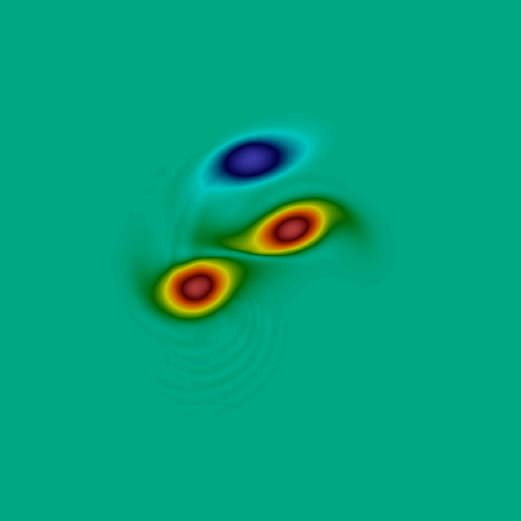
\includegraphics[scale=0.06]{data/Incompressible_Euler/Snapshots/red_17_2.png}\hspace{1em}
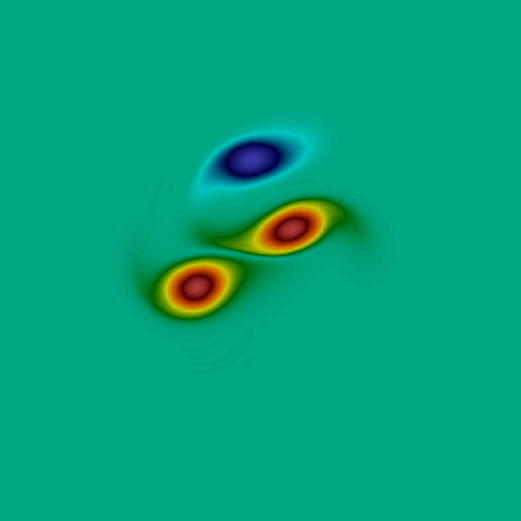
\includegraphics[scale=0.06]{data/Incompressible_Euler/Snapshots/red_35_2.png}\hspace{1em}
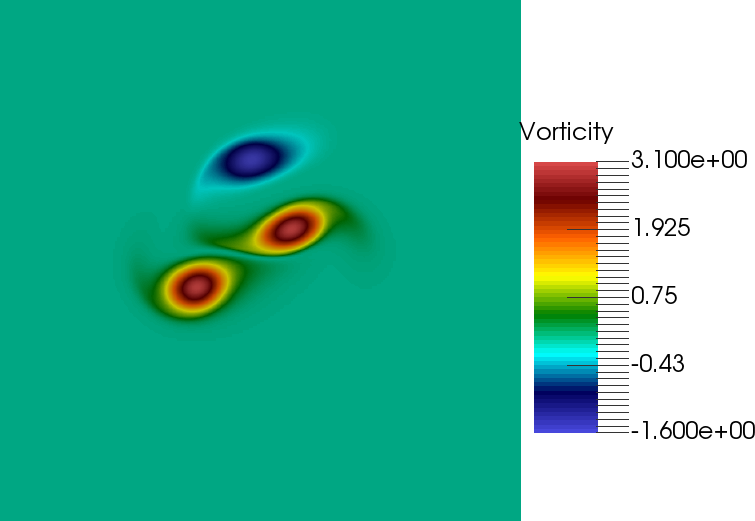
\includegraphics[scale=0.06]{data/Incompressible_Euler/Snapshots/Full_2.png}\\

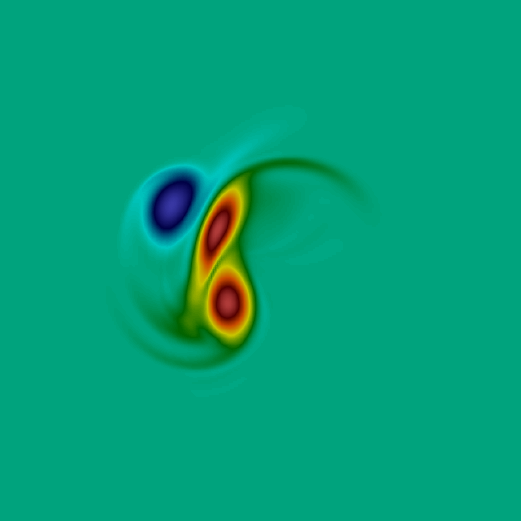
\includegraphics[scale=0.06]{data/Incompressible_Euler/Snapshots/red_17_3.png}\hspace{1em}
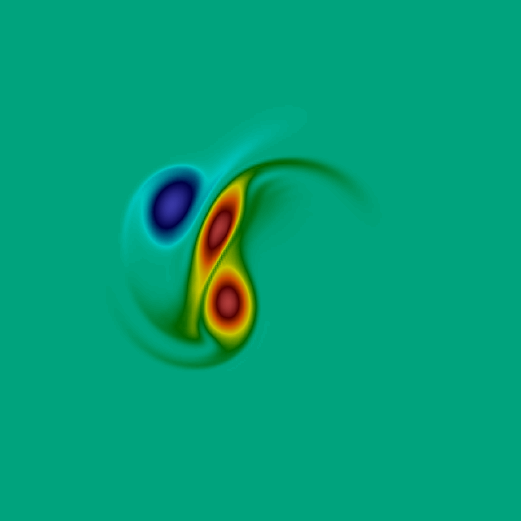
\includegraphics[scale=0.06]{data/Incompressible_Euler/Snapshots/red_35_3.png}\hspace{1em}
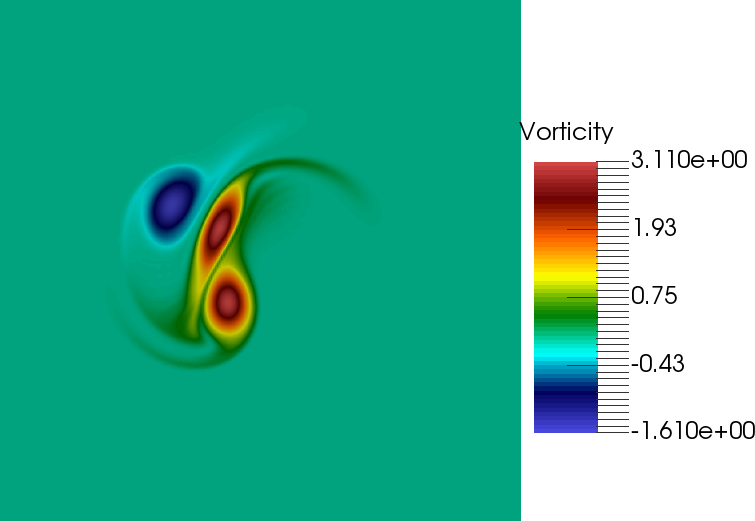
\includegraphics[scale=0.06]{data/Incompressible_Euler/Snapshots/Full_3.png}\\

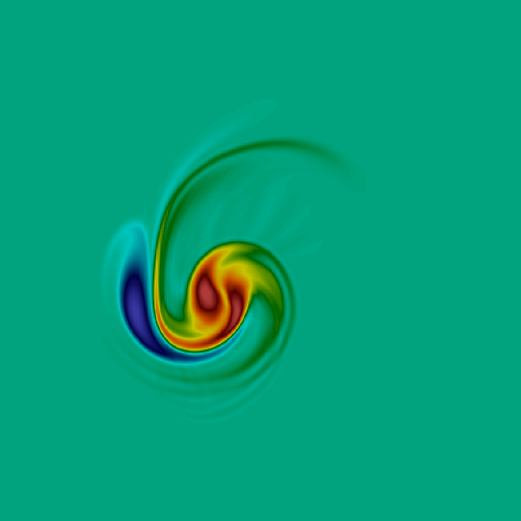
\includegraphics[scale=0.06]{data/Incompressible_Euler/Snapshots/red_17_4.png}\hspace{1em}
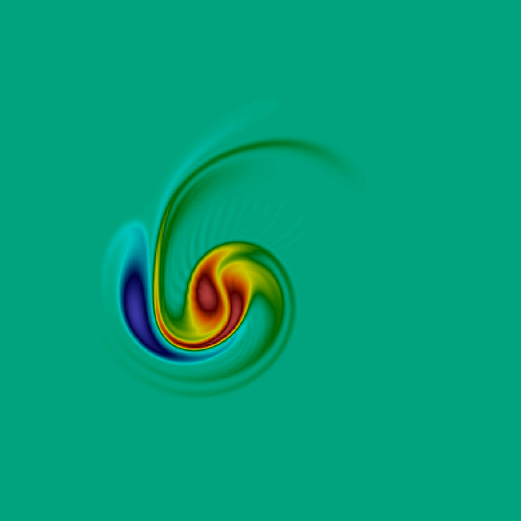
\includegraphics[scale=0.06]{data/Incompressible_Euler/Snapshots/red_35_4.png}\hspace{1em}
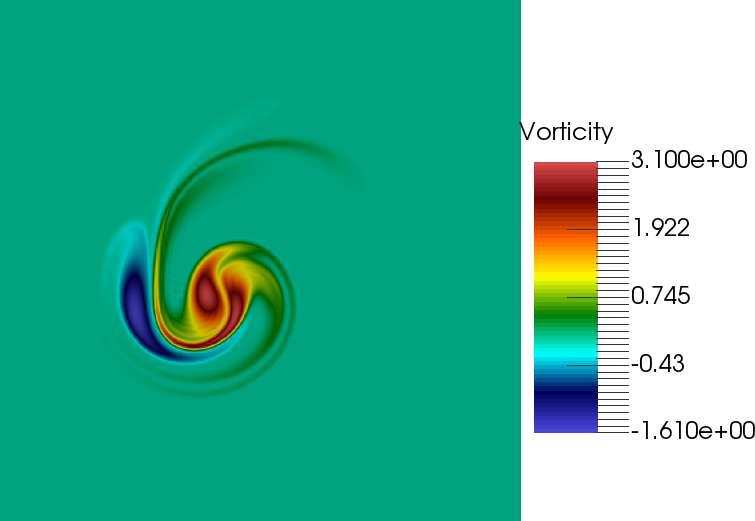
\includegraphics[scale=0.06]{data/Incompressible_Euler/Snapshots/Full_4.png}\\

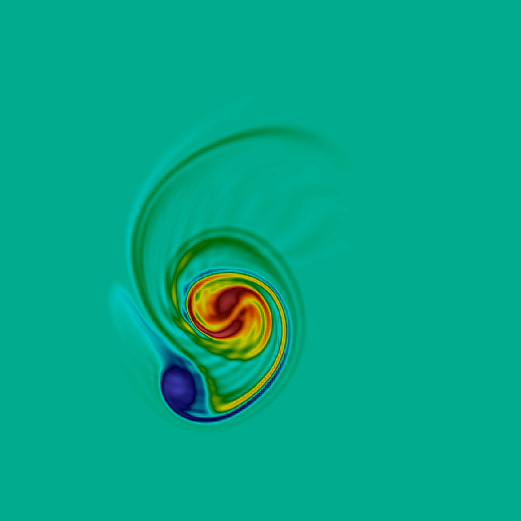
\includegraphics[scale=0.06]{data/Incompressible_Euler/Snapshots/red_17_5.png}\hspace{1em}
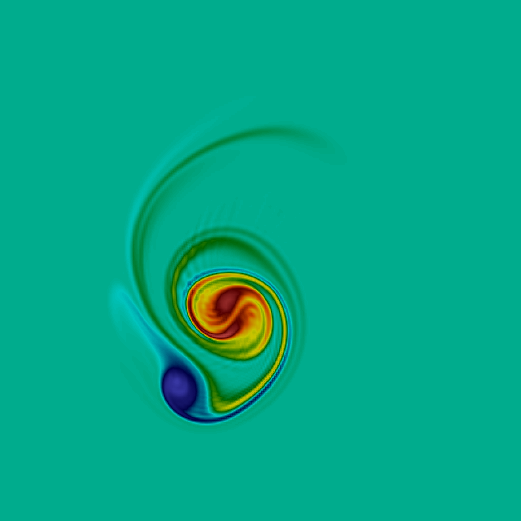
\includegraphics[scale=0.06]{data/Incompressible_Euler/Snapshots/red_35_5.png}\hspace{1em}
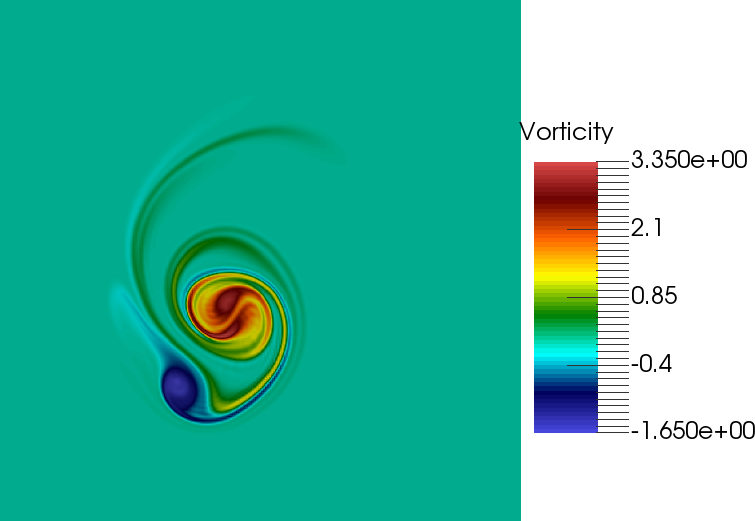
\includegraphics[scale=0.06]{data/Incompressible_Euler/Snapshots/Full_5.png}

\caption{Snapshots of the high-fidelity system and the reduced system at $t=\left\{ 4,8,12,18 \right\}$. From left to right: the solution of the reduced model with $k=17$, $k=35$ and the high fidelity solution.}
\label{fig:snap_solution_incompressible_Euler}
\end{figure}


%%%%%%%%%%%%%%%%%%%%%%%%%%%%%%%%%%%%%%%%%%
%%%%%%%%%% Singular values decay merging vorteces %%%%%%%%%%%
%%%%%%%%%%%%%%%%%%%%%%%%%%%%%%%%%%%%%%%%%%
\Cref{fig:approx_error_incompressible_Euler} shows the $L^2$ error between the high-fidelity solution and the reduced solution. The error decreases, consistently, as the number of basis vectors increases. Furthermore, the accuracy is maintained over the period of time integration.

The conservation of the kinetic energy is presented in \Cref{fig:energy_error_incompressible_Euler}. Even for a small number of basis vectors, where the solution is not well approximated, the kinetic energy remains constant. Furthermore, the error in the kinetic energy, due to MOR, is constant in time. This is central for the robustness of the reduced system during long time-integration.


%%%%%%%%%%%%%%%%%%%%%%%%%%%%%%%%%%%%%%%%%%%
%%%%%%%%%% Approximation error and energy conservation %%%%%%%%%%
%%%%%%%%%%%%%%%%%%%%%%%%%%%%%%%%%%%%%%%%%%%
\begin{figure}[t]
\centering
\begin{subfigure}[]{0.47\linewidth}
\begin{tikzpicture}[scale=0.58]
    \begin{semilogyaxis}[ylabel = $\| \mathbf{u}-\tilde{\mathbf{u}}\|_2$,
                 xlabel=$t$,
                 label style={font=\Large},
                 legend style={font=\large},
                 grid=both,
                 ticks=both,
                 width=1.4\linewidth, 
                 height=1.0\linewidth,
                 minor x tick num=1,
                 minor y tick num=2,	
                 yticklabel style={/pgf/number format/.cd,fixed,precision=9},
                 scaled x ticks = true,
                 enlargelimits=false,
                 scale only axis,
                 samples = 100,
                 cycle list name=exotic]
                 \addplot+[style=solid,style=ultra thick]  table[x = time, y = error] {./data/Incompressible_Euler/Approximation_Error/err_5.txt};
                 \addplot+[style=solid,style=ultra thick]  table[x = time, y = error] {./data/Incompressible_Euler/Approximation_Error/err_8.txt};
                 \addplot+[style=solid,style=ultra thick]  table[x = time, y = error] {./data/Incompressible_Euler/Approximation_Error/err_11.txt};
                 \addplot+[style=solid,style=ultra thick]  table[x = time, y = error] {./data/Incompressible_Euler/Approximation_Error/err_14.txt};
                 \addplot+[style=solid,style=ultra thick]  table[x = time, y = error] {./data/Incompressible_Euler/Approximation_Error/err_23.txt};
                 \addplot+[style=solid,style=ultra thick]  table[x = time, y = error] {./data/Incompressible_Euler/Approximation_Error/err_26.txt};
                 \addplot+[style=solid,style=ultra thick]  table[x = time, y = error] {./data/Incompressible_Euler/Approximation_Error/err_29.txt};
                 \addplot+[style=solid,style=ultra thick]  table[x = time, y = error] {./data/Incompressible_Euler/Approximation_Error/err_35.txt};
    \end{semilogyaxis}
\end{tikzpicture}
\caption{}
\label{fig:approx_error_incompressible_Euler}
\end{subfigure} \hfill
\begin{subfigure}[]{0.47\linewidth}
\begin{tikzpicture}[scale=0.58]
    \begin{axis}[ylabel = $|K-\tilde{K}|$,
                 xlabel=$t$,
                 label style={font=\Large},
                 legend pos=south west,
                 legend entries={$k=5$ , $k=8$, $k=11$, $k=14$, $k=23$, $k=26$, $k=29$, $k=35$},
                 legend style={font=\large},
                 grid=both,
                 ticks=both,
                 width=1.4\linewidth, 
                 height=1.0\linewidth,
                 minor x tick num=1,
                 minor y tick num=2,	
                 yticklabel style={/pgf/number format/.cd,fixed,precision=9},
                 scaled x ticks = true,
                 enlargelimits=false,
                 scale only axis,
                 ymax = 0.5598,
                 samples = 100,
                 cycle list name=exotic]
                 \addplot+[style=solid,style=ultra thick]  table[x = time, y = error] {./data/Incompressible_Euler/Energy_conservation/ene_full_5.txt};
                 \addplot+[style=solid,style=ultra thick]  table[x = time, y = error] {./data/Incompressible_Euler/Energy_conservation/ene_full_8.txt};
                 \addplot+[style=solid,style=ultra thick]  table[x = time, y = error] {./data/Incompressible_Euler/Energy_conservation/ene_full_11.txt};
                 \addplot+[style=solid,style=ultra thick]  table[x = time, y = error] {./data/Incompressible_Euler/Energy_conservation/ene_full_14.txt};
                 \addplot+[style=solid,style=ultra thick]  table[x = time, y = error] {./data/Incompressible_Euler/Energy_conservation/ene_full_23.txt};
                 \addplot+[style=solid,style=ultra thick]  table[x = time, y = error] {./data/Incompressible_Euler/Energy_conservation/ene_full_26.txt};
                 \addplot+[style=solid,style=ultra thick]  table[x = time, y = error] {./data/Incompressible_Euler/Energy_conservation/ene_full_29.txt};
                 \addplot+[style=solid,style=ultra thick]  table[x = time, y = error] {./data/Incompressible_Euler/Energy_conservation/ene_full_35.txt};
    \end{axis}
\end{tikzpicture}
\caption{}
\label{fig:energy_error_incompressible_Euler}
\end{subfigure}
\label{fig:energy_approx_err}
\caption{(\protect\subref{fig:approx_error_incompressible_Euler}) Evolution of $L_2$ error in velocity, between the high-fidelity system and the reduced system. (\protect\subref{fig:energy_error_incompressible_Euler}) Conservation of the kinetic energy.}
\end{figure}


\subsection{2D Kelvin-Helmholtz instability}
Consider the 2-dimensional compressible Euler equation \eqref{eq:3.18} in a periodic square box $[0,1]^2$. Unlike the incompressible example in \Cref{sec:res.1}, a centered finite difference scheme of fourth order is used to discretize \eqref{eq:3.18}. The physical domain is discretized into a grid of $256\times 256$ nodes.

The initial velocity field is given by
\begin{equation*}
\begin{cases}
& \mathbf{r} = 
\begin{cases}
& 2, \text{ if } 0.25<y<0.75,\\
& 1, \text{ otherwise },
\end{cases}
\\
& \mathbf{u}_x = a \sin(4\pi y) \left( e^{-\dfrac{(y-0.25)^2}{2\sigma^2}} + e^{-\dfrac{(y-0.75)^2}{2\sigma^2}} \right),\\
& \mathbf{u}_y = 
\begin{cases}
& 0.5, \text{ if } 0.25<y<0.75,\\
& -0.5, \text{ otherwise },
\end{cases},
\\
& \mathbf{p} = 2.5,\\
\end{cases}
\end{equation*}
where $a=0.1$ and $\sigma=5\sqrt{2}\cdot 10^{-3}$. This corresponds to contacting streams of fluid with different densities. For specific choices of parameters describing the jets, fine structures and vortices emerges at the interface between the streams. Such an instability is referred to as the Kelvin-Helmholtz instability \cite{HHS}.

As centered schemes are often dissipation free, resolving the discontinuous initial data requires some artificial viscosity. In the high-fidelity model, the method discussed in \cite{artificial_dissipation}\edit{, based on a derivative-based model,} is used as an artificial viscosity. However, at the level of the reduced system, this is replaced with a low pass filter on the expansion coefficients of POD basis vectors. \edit{The last $5\%$ of the POD modes are put to zero at each time iteration. The reason for the different treatment is that we want to avoid the reconstruction of the derivative of the solution in the full space during the integration of the reduced system.}

The fully discrete skew-symmetric form \eqref{eq:3.27} is used as a time marching scheme with $\Delta t = 5 \cdot 10^{-4}$ over a period of $1$ time unit.
\edit{A total of $500$ snapshots have been used for the computation of the basis in the offline stage.}

\Cref{fig:error_decay_KH} illustrates that the accuracy of the method consistently improves as a higher number of POD basis modes are considered. Furthermore, the skew-symmetric form preserves the accuracy over the period of time integration. It is observed in \Cref{fig:snap_solution_KH} that all features of the flow are correctly represented in the reduced system, even with a low number of basis vectors.

\begin{figure}[t]
\centering
\begin{subfigure}[]{0.48\linewidth}
  \begin{tikzpicture}[scale=0.55]
    \begin{semilogyaxis}[xlabel=$t$,
                 ylabel=$e(t)$,
                 label style={font=\Large},
                 legend pos=outer north east,
                 legend style={font=\large},
                 legend entries={$k=200$,$k=300$,$k=400$,$k=500$,$k=600$},
                 grid=both,
                 ticks=both,
                 width=1.4\linewidth, 
                 height=1.0\linewidth,
                 minor x tick num=1,
                 minor y tick num=2,	
                 yticklabel style={/pgf/number format/.cd,fixed,precision=9},
                 scaled x ticks = true,
                 enlargelimits=false,
                 scale only axis,
                 cycle list name=exotic]
                 \addplot+[style=solid,style=ultra thick]  table[x = time, y = quantity] {./data/Compressible_Euler/KH/error/error_200.txt};  
                 \addplot+[style=solid,style=ultra thick]  table[x = time, y = quantity] {./data/Compressible_Euler/KH/error/error_300.txt};      
                 \addplot+[style=solid,style=ultra thick]  table[x = time, y = quantity] {./data/Compressible_Euler/KH/error/error_400.txt}; 
                 \addplot+[style=solid,style=ultra thick]  table[x = time, y = quantity] {./data/Compressible_Euler/KH/error/error_500.txt};      
                 \addplot+[style=solid,style=ultra thick]  table[x = time, y = quantity] {./data/Compressible_Euler/KH/error/error_600.txt};               
    \end{semilogyaxis}%  
  \end{tikzpicture}
\end{subfigure}
\caption{Evolution in time of the error  between the high fidelity solution of the Kelvin-Helmoltz and the reduced solution for different number of basis $k$. As error measure we use $e(t)=\sqrt{\|\mathbf{r}-\mathbf{r}^r\|^2+\|\mathbf{u_xr}-\mathbf{u_xr}^r\|^2 + \|\mathbf{u_yr}-\mathbf{u_yr}^r\|^2 + \|\mathbf{p}-\mathbf{p}^r\|^2}$.}
\label{fig:error_decay_KH}
\end{figure}

Conservation of mass, momentum and energy is presented in \Cref{fig:conservation_DEIM}. The accuracy of the method in approximating these invariants improves as the size of the basis is increased. Furthermore, \Cref{energy_error_KH} shows how the kinetic energy associated with the reduced system mimic the kinetic energy of the high-fidelity system. This helps to ensure the correct evolution of kinetic energy, and thus, the internal energy.
 
\begin{figure}
  \centering
  \begin{subfigure}[]{0.48\linewidth}
  \begin{tikzpicture}[scale=0.55]
    \begin{semilogyaxis}[ylabel = error in mass,
                 xlabel=$t$,
                 label style={font=\Large},
                 legend pos=north east,
                 legend entries={$k=200$ ,$k=300$, $k=400$,$k=500$,$k=600$},
                 legend style={font=\large},
                 grid=both,
                 ticks=both,
                 width=1.4\linewidth, 
                 height=1.0\linewidth,
                 minor x tick num=1,
                 minor y tick num=2,	
                 %yticklabel style={/pgf/number format/.cd,fixed,precision=9},
                 scaled x ticks = true,
                 enlargelimits=false,
                 scale only axis,
                 cycle list name=exotic]
                 \addplot+[style=solid,style=ultra thick]  table[x = time, y = quantity] {./data/Compressible_Euler/KH/conserved_quantities/mass_red_200.txt};
                 \addplot+[style=solid,style=ultra thick]  table[x = time, y = quantity] {./data/Compressible_Euler/KH/conserved_quantities/mass_red_300.txt};
                 \addplot+[style=solid,style=ultra thick]  table[x = time, y = quantity] {./data/Compressible_Euler/KH/conserved_quantities/mass_red_400.txt};
                 \addplot+[style=solid,style=ultra thick]  table[x = time, y = quantity] {./data/Compressible_Euler/KH/conserved_quantities/mass_red_500.txt};
                 \addplot+[style=solid,style=ultra thick]  table[x = time, y = quantity] {./data/Compressible_Euler/KH/conserved_quantities/mass_red_600.txt};
    \end{semilogyaxis}%  
  \end{tikzpicture}
  \caption{}
  \label{mass_error_KH}
  \end{subfigure}\hfill
  \begin{subfigure}[]{0.48\linewidth}
  \begin{tikzpicture}[scale=0.55]
    \begin{semilogyaxis}[ylabel = error in total momentum,
                 xlabel=$t$,
                 label style={font=\Large},
                 legend pos=north east,
%                 legend entries={$k=200$ Conv,$k=201$ Conv},
                 legend style={font=\large},
                 grid=both,
                 ticks=both,
                 width=1.4\linewidth, 
                 height=1.0\linewidth,
                 minor x tick num=1,
                 minor y tick num=2,	
                 %yticklabel style={/pgf/number format/.cd,fixed,precision=9},
                 scaled x ticks = true,
                 enlargelimits=false,
                 scale only axis,
                 cycle list name=exotic]
                 \addplot+[style=solid,style=ultra thick]  table[x = time, y = quantity] {./data/Compressible_Euler/KH/conserved_quantities/momentum_red_200.txt};
                 \addplot+[style=solid,style=ultra thick]  table[x = time, y = quantity] {./data/Compressible_Euler/KH/conserved_quantities/momentum_red_300.txt};
                 \addplot+[style=solid,style=ultra thick]  table[x = time, y = quantity] {./data/Compressible_Euler/KH/conserved_quantities/momentum_red_400.txt};
                 \addplot+[style=solid,style=ultra thick]  table[x = time, y = quantity] {./data/Compressible_Euler/KH/conserved_quantities/momentum_red_500.txt};
                 \addplot+[style=solid,style=ultra thick]  table[x = time, y = quantity] {./data/Compressible_Euler/KH/conserved_quantities/momentum_red_600.txt};
    \end{semilogyaxis}%  
  \end{tikzpicture}
  \caption{}
  \label{momentum_error_KH}
  \end{subfigure}
  
  \begin{subfigure}[]{0.48\linewidth}
  \begin{tikzpicture}[scale=0.55]
    \begin{semilogyaxis}[ylabel = error in total energy,
                 xlabel=$t$,
                 label style={font=\Large},
                 legend pos=north east,
%                 legend entries={$k=200$ Conv,$k=201$ Conv},
                 legend style={font=\large},
                 grid=both,
                 ticks=both,
                 width=1.4\linewidth, 
                 height=1.0\linewidth,
                 minor x tick num=1,
                 minor y tick num=2,	
                 %yticklabel style={/pgf/number format/.cd,fixed,precision=9},
                 scaled x ticks = true,
                 enlargelimits=false,
                 scale only axis,
                 cycle list name=exotic]
                 \addplot+[style=solid,style=ultra thick]  table[x = time, y = quantity] {./data/Compressible_Euler/KH/conserved_quantities/energy_red_200.txt};
                 \addplot+[style=solid,style=ultra thick]  table[x = time, y = quantity] {./data/Compressible_Euler/KH/conserved_quantities/energy_red_300.txt};
                 \addplot+[style=solid,style=ultra thick]  table[x = time, y = quantity] {./data/Compressible_Euler/KH/conserved_quantities/energy_red_400.txt};
                 \addplot+[style=solid,style=ultra thick]  table[x = time, y = quantity] {./data/Compressible_Euler/KH/conserved_quantities/energy_red_500.txt};
                 \addplot+[style=solid,style=ultra thick]  table[x = time, y = quantity] {./data/Compressible_Euler/KH/conserved_quantities/energy_red_600.txt};
    \end{semilogyaxis}%  
  \end{tikzpicture}
   \caption{}
  \label{energy_error_KH}
  \end{subfigure}
\caption{Difference between the high fidelity solution of the Kelvin-Helmholtz problem and the reduced solution of the mass (\protect\subref{mass_error_KH}), the momentum (\protect\subref{momentum_error_KH}), and the total energy (\protect\subref{energy_error_KH}).}
\label{fig:conservation_DEIM}
\end{figure}

%%%%%%%%%%%%%%%%%%%%%%%%%%%%%%%%%%%%%
%%%%%%%%%%%%%% Snapshots of KH %%%%%%%%%%%%%%
%%%%%%%%%%%%%%%%%%%%%%%%%%%%%%%%%%%%%
\begin{figure}[h!]
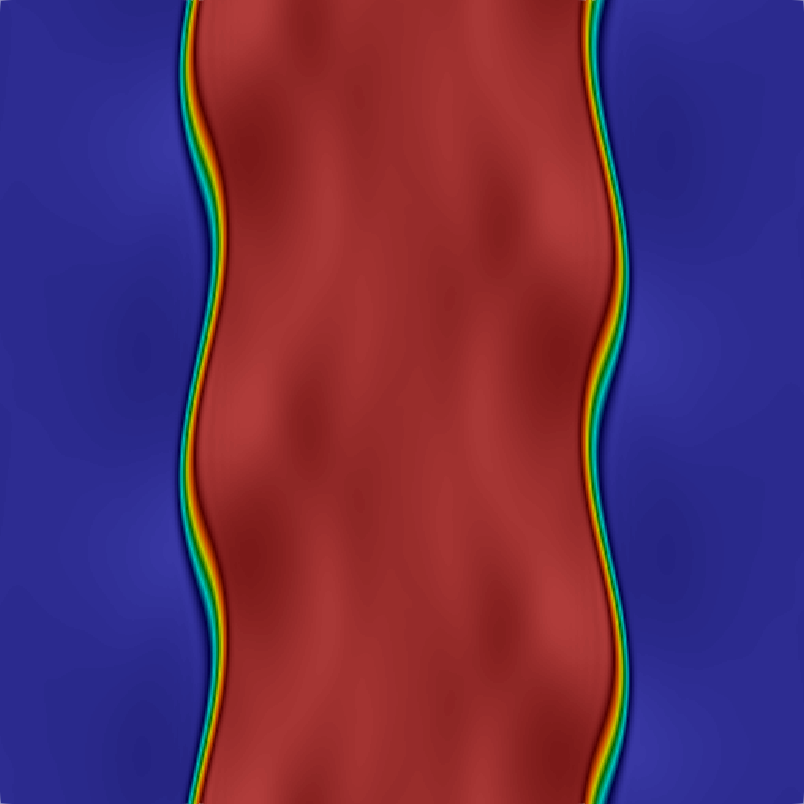
\includegraphics[scale=0.115]{data/Compressible_Euler/KH/Snapshots/density_200_307.png}\hspace{1em}
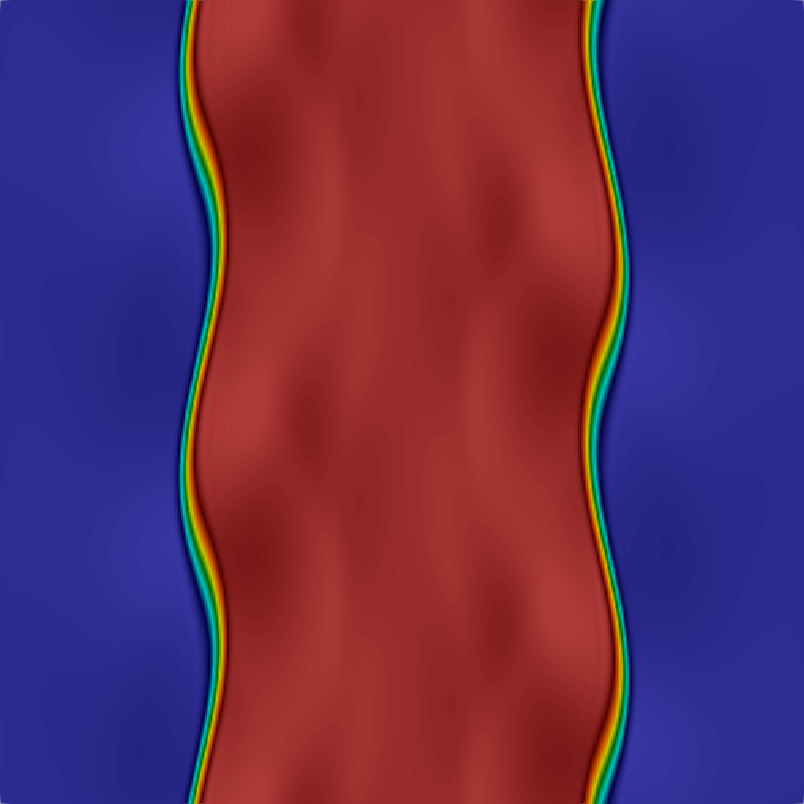
\includegraphics[scale=0.115]{data/Compressible_Euler/KH/Snapshots/density_500_307.png}\hspace{1em}
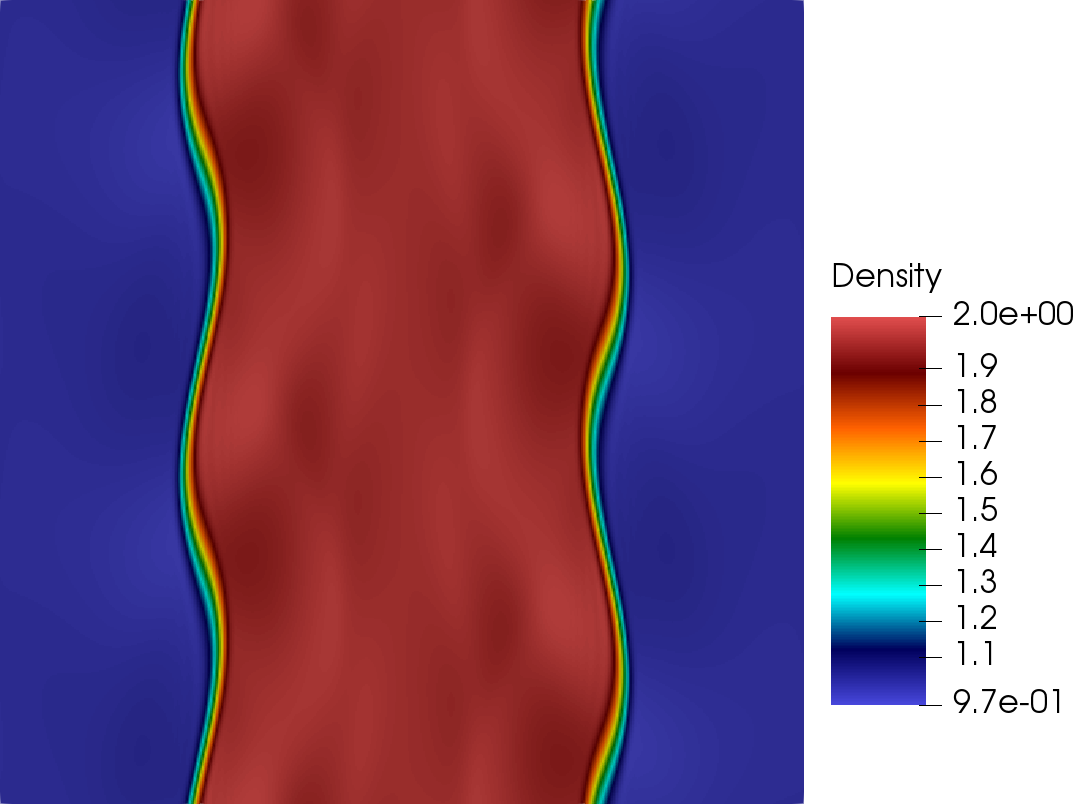
\includegraphics[scale=0.115]{data/Compressible_Euler/KH/Snapshots/density_exact_307.png}\\

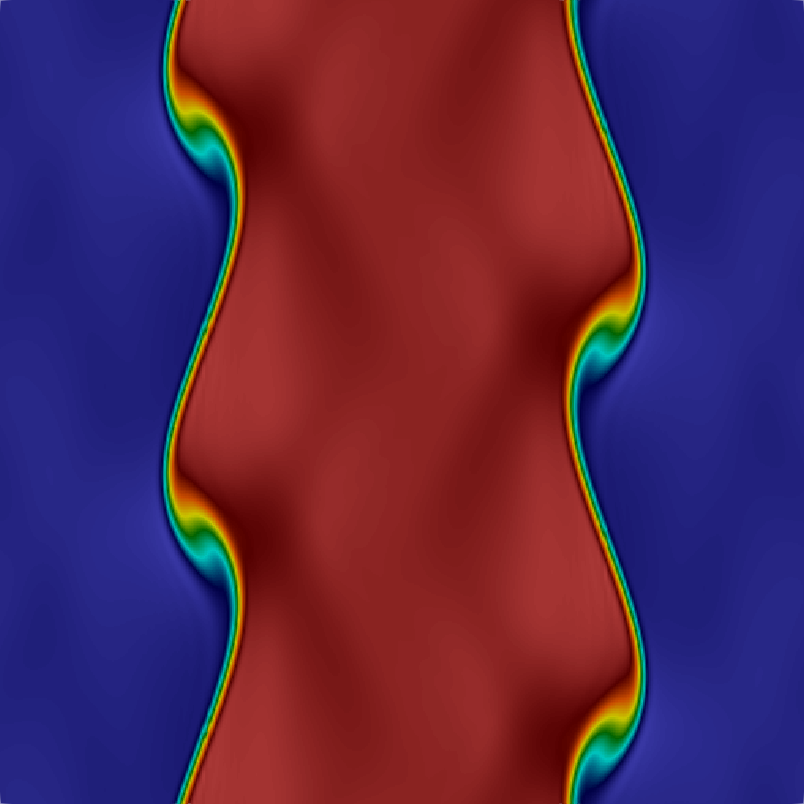
\includegraphics[scale=0.115]{data/Compressible_Euler/KH/Snapshots/density_200_461.png}\hspace{1em}
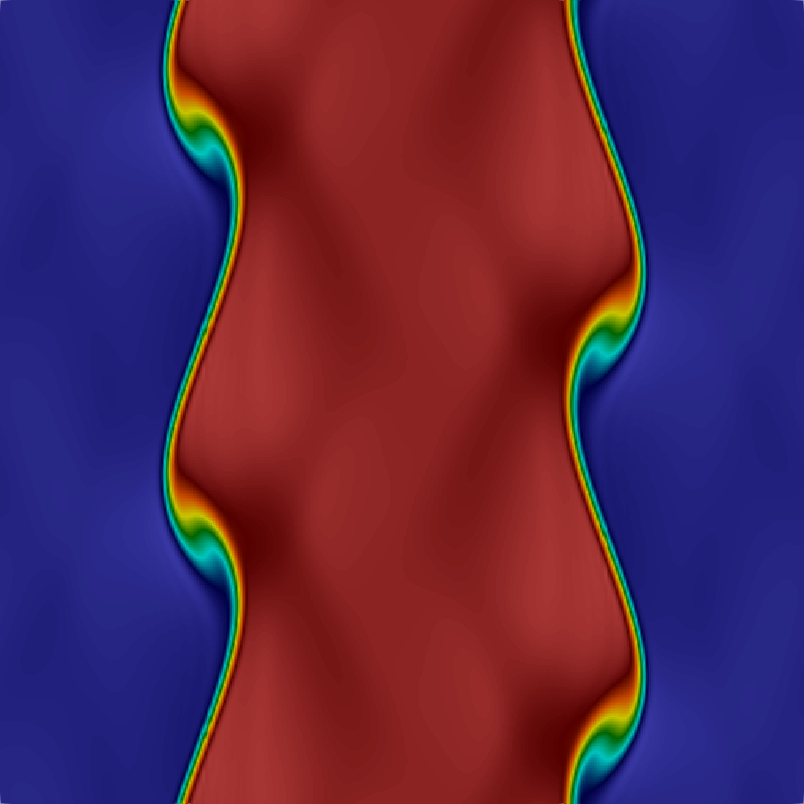
\includegraphics[scale=0.115]{data/Compressible_Euler/KH/Snapshots/density_500_461.png}\hspace{1em}
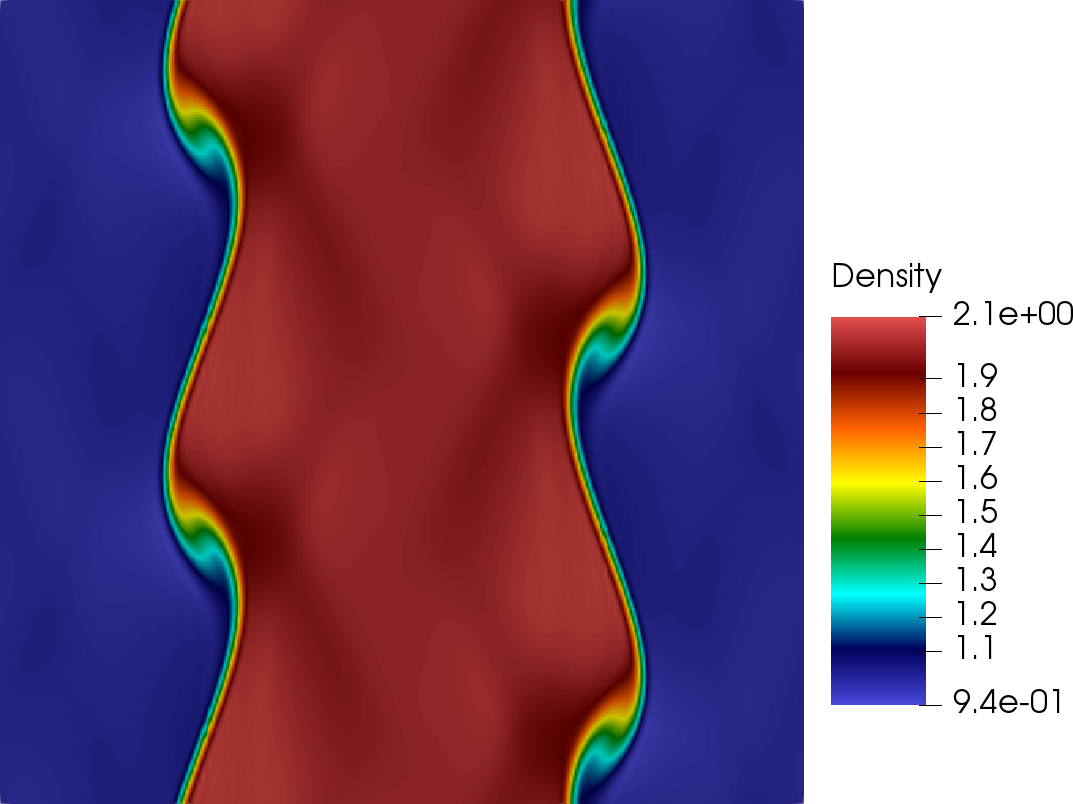
\includegraphics[scale=0.115]{data/Compressible_Euler/KH/Snapshots/density_exact_461.png}\\


\includegraphics[scale=0.115]{data/Compressible_Euler/KH/Snapshots/density_200_614.png}\hspace{1em}

\includegraphics[scale=0.115]{data/Compressible_Euler/KH/Snapshots/density_500_614.png}\hspace{1em}
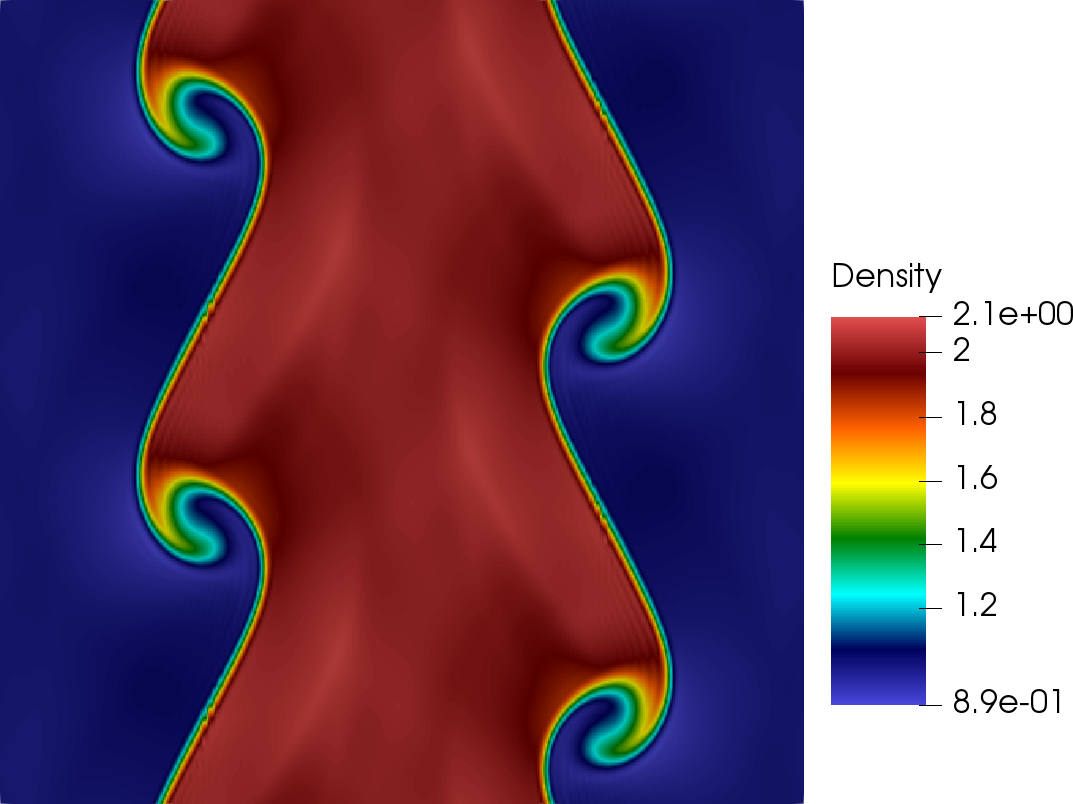
\includegraphics[scale=0.115]{data/Compressible_Euler/KH/Snapshots/density_exact_614.png}\\


\includegraphics[scale=0.115]{data/Compressible_Euler/KH/Snapshots/density_200_768.png}\hspace{1em}

\includegraphics[scale=0.115]{data/Compressible_Euler/KH/Snapshots/density_500_768.png}\hspace{1em}
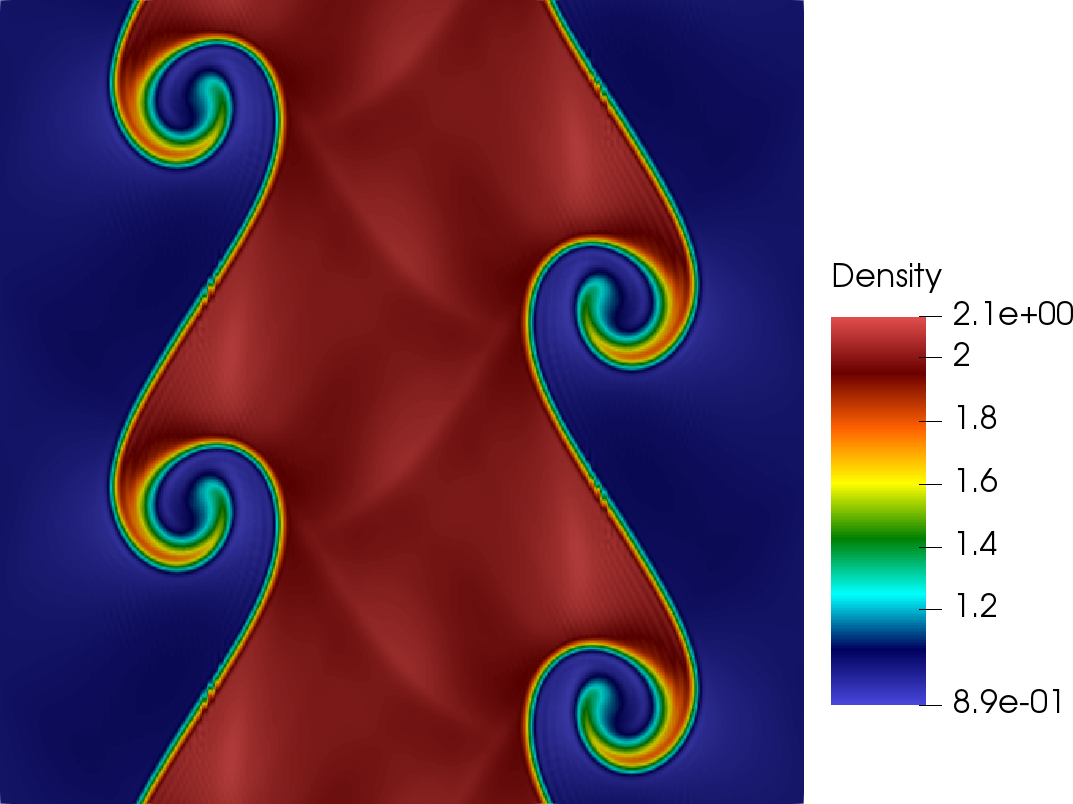
\includegraphics[scale=0.115]{data/Compressible_Euler/KH/Snapshots/density_exact_768.png}

\caption{Solutions of the Kelvin-Helmholtz problem at $t=\left\{ 0.4, 0.6, 0.8, 1 \right\}$. From left to right we show the solution of the reduced model with $k=200$, $k=500$ and the high fidelity solution.}
\label{fig:snap_solution_KH}
\end{figure}


\subsection{1D Shock problem}
In this section we study the 1-dimensional compressible Euler problem, \eqref{eq:3.18} without viscous terms, with a steady state discontinuous solution. This is in preparation for \Cref{sec:5.res.4}, where development and propagation of shock waves is discussed. Here we asses how the skew-symmetric form of \eqref{eq:3.18} can recover moving discontinuities at the level of the reduced system. Consider a periodic boundary conditions on $\Omega = [0,1]$ with the initial condition
\begin{equation*}
\begin{cases}
& \mathbf{r} = 0.5+0.2 \cos(2\pi x),\\
& \mathbf{u} = 1.5,\\
& \mathbf{p} = 0.5+0.2 \sin(2\pi x).\\
\end{cases}
\end{equation*}
The domain is discretized into $N=2000$ nodes and a centered finite differences scheme is used to assemble the discrete Euler equation in skew-symmetric form, as discussed in \Cref{sec:skew.3}. 

The fully discrete skew-symmetric form \eqref{eq:3.27} is used for time integration over a time interval $[0,0.3]$. To resolve the discontinuous solution we use an artificial viscosity with $\tau = \mu \partial u / \partial x$, where $\mu = 0.5 \cdot 10^{-4}$. \edit{Regarding the reduction procedure, $1000$ snapshots of the numerical solution given by the high fidelity method have been collected.}

		\Cref{fig:energy_pres_1D} shows the evolution of conserved quantities for the high-fidelity and reduced system. Here, the high-fidelity model is also considered in the divergence and advective form in addition to the skew-symmetric form. It is clear that when the reduced systems is not in skew-symmetric form, it violates conservation of mass, momentum, and energy. Even while the high-fidelity systems in divergence and advective forms are stable, the constructed reduced system is unstable, independent on the number of basis vectors. On the other hand, the skew-symmetric form yields a stable and conservative reduce system. Note that the loss in the energy associated with the skew-symmetric form, illustrated in \Cref{conservation_1D_focus}, is due to the application of an artificial viscosity. 

\Cref{error_behaviour_1D} shows the total error, when the reduced system captures a discontinuous solution at $t=0.16$. It is observed that the formation of a discontinuity affects the accuracy of the method. This is expected as a sharp gradient is approximated by a relatively few POD modes. However, the method remains robust and stable during the period of time integration.

In \Cref{fig:snaps_1D_Euler} we compare the numerical artifacts of different formulations of the Euler equation. The advective formulation is not presented since it does not yield a stable reduced system. It is observed that the reduced system based on the skew-symmetric formulation accurately represent the overall behavior of the high-fidelity solution. On the other hand, a Gibbs-type error \cite{thompson1992fourier} appears near sharp gradients, for the reduced system based on the divergence form of the Euler equation. The well-representation of the skew-symmetric form is due the low aliasing error property. 

As discussed in \Cref{sec:mor_skew}, the DEIM approximation needed for an efficient evaluation of the nonlinear components of \eqref{eq:3.18}, can affect the conservation properties of the skew-symmetric form. \Cref{fig:singular_values_decay_1D} shows the decay of the singular values of the nonlinear snapshots. The decay of these snapshots is significantly slower than the temporal snapshots of \eqref{eq:3.18}. This indicates that to maintain the accuracy of the reduced system, the DEIM basis should be chosen richer than the POD basis. \Cref{error_DEIM} and \Cref{energy_DEIM} present the error and the conservation of total energy when the DEIM is used to approximate the nonlinear term. The conservation of energy is recovered once DEIM approximates the nonlinear terms with enough accuracy. 
In this numerical experiment, evaluation of the nonlinear terms in \eqref{eq:3.18} using the DEIM is ten times faster than the high-fidelity evaluation.

%%%%%%%%%%%%%%%%%%%%%%%%%%%%%%%%%%%%%%%%%%%%
%%%%%%%%%%%%% Mass, Total momentum & Energy %%%%%%%%%%%%%%
%%%%%%%%%%%%%%%%%%%%%%%%%%%%%%%%%%%%%%%%%%%%
\begin{figure}
  \centering
  % MASS
  \begin{subfigure}[]{0.48\linewidth}
  \begin{tikzpicture}[scale=0.55]
    \begin{axis}[ylabel = Mass,
                 xlabel=$t$,
                 label style={font=\Large},
                 legend pos=north east,
                 legend entries={$k=102$ Adv,$k=201$ Adv,$k=102$ Div,$k=201$ Div,$k=102$ Skew,$k=201$ Skew},
                 legend style={font=\large},
                 grid=both,
                 ticks=both,
                 width=1.4\linewidth, 
                 height=1.0\linewidth,
                 minor x tick num=1,
                 minor y tick num=2,	
                 yticklabel style={/pgf/number format/.cd,fixed,precision=9},
                 scaled x ticks = true,
                 enlargelimits=false,
                 scale only axis,
                 ymin=0,
                 ymax = 2,
                 samples = 100]
                 \addplot[color=red,style=dashdotted,style=ultra thick]  table[x = time, y = quantity] {./data/Compressible_Euler/1D/convective_data/mass_102_1.txt};
                 \addplot[color=blue,style=dashdotted,style=ultra thick]  table[x = time, y = quantity] {./data/Compressible_Euler/1D/convective_data/mass_201_1.txt};
                 \addplot[color=red,style=dashed,style=ultra thick]  table[x = time, y = quantity] {./data/Compressible_Euler/1D/divergence_data/mass_102_1.txt};
                 \addplot[color=blue,style=dashed,style=ultra thick]  table[x = time, y = quantity] {./data/Compressible_Euler/1D/divergence_data/mass_201_1.txt};
                 \addplot[color=red,style=solid,style=ultra thick]  table[x = time, y = quantity] {./data/Compressible_Euler/1D/skew_symm_data/mass_102_1.txt};
                 \addplot[color=blue,style=solid,style=ultra thick]  table[x = time, y = quantity] {./data/Compressible_Euler/1D/skew_symm_data/mass_201_1.txt};
    \end{axis}%  
  \end{tikzpicture}
  \end{subfigure}\hfill% 
  % MASS (focus)
  \begin{subfigure}[]{0.48\linewidth}
  \begin{tikzpicture}[scale=0.55]
    \begin{axis}[xlabel=$t$,
                 label style={font=\Large},
                 legend pos=south west,
                 legend entries={$k=24$ Skew,$k=102$ Skew,$k=201$ Skew},
                 legend style={font=\large},
                 grid=both,
                 ticks=both,
                 width=1.4\linewidth, 
                 height=1.0\linewidth,
                 minor x tick num=1,
                 minor y tick num=2,	
                 yticklabel style={/pgf/number format/.cd,fixed,precision=9},
                 scaled x ticks = true,
                 enlargelimits=false,
                 scale only axis,
                 ymax=0.5000001]
                 \addplot[color=black!50!green,style=solid,style=ultra thick]  table[x = time, y = quantity] {./data/Compressible_Euler/1D/skew_symm_data/mass_24_1.txt};
                 \addplot[color=red,style=solid,style=ultra thick]  table[x = time, y = quantity] {./data/Compressible_Euler/1D/skew_symm_data/mass_102_1.txt};
                 \addplot[color=blue,style=solid,style=ultra thick]  table[x = time, y = quantity] {./data/Compressible_Euler/1D/skew_symm_data/mass_201_1.txt};
    \end{axis}%  
  \end{tikzpicture}
  \end{subfigure}
 % TOTAL MOMENTUM
  \begin{subfigure}[]{0.48\linewidth}
  \begin{tikzpicture}[scale=0.55]
    \begin{axis}[ylabel = Momentum,
                 xlabel=$t$,
                 label style={font=\Large},
                 legend pos=north east,
                 %legend entries={$k=24$ Div,$k=102$ Div,$k=201$ Div,$k=24$ Skew,$k=102$ Skew,$k=201$ Skew},
                 legend style={font=\large},
                 grid=both,
                 ticks=both,
                 width=1.4\linewidth, 
                 height=1.0\linewidth,
                 minor x tick num=1,
                 minor y tick num=2,	
                 yticklabel style={/pgf/number format/.cd,fixed,precision=9},
                 scaled x ticks = true,
                 enlargelimits=false,
                 scale only axis,
                 ymin=1,
                 ymax = 2,
                 samples = 100]
                 \addplot[color=red,style=dashdotted,style=ultra thick]  table[x = time, y = quantity] {./data/Compressible_Euler/1D/convective_data/momentum_102_1.txt};
                 \addplot[color=blue,style=dashdotted,style=ultra thick]  table[x = time, y = quantity] {./data/Compressible_Euler/1D/convective_data/momentum_201_1.txt};
                 \addplot[color=red,style=dashed,style=ultra thick]  table[x = time, y = quantity] {./data/Compressible_Euler/1D/divergence_data/momentum_102_1.txt};
                 \addplot[color=blue,style=dashed,style=ultra thick]  table[x = time, y = quantity] {./data/Compressible_Euler/1D/divergence_data/momentum_201_1.txt};
                 \addplot[color=red,style=solid,style=ultra thick]  table[x = time, y = quantity] {./data/Compressible_Euler/1D/skew_symm_data/momentum_102_1.txt};
                 \addplot[color=blue,style=solid,style=ultra thick]  table[x = time, y = quantity] {./data/Compressible_Euler/1D/skew_symm_data/momentum_201_1.txt};
    \end{axis}%  
  \end{tikzpicture} 
  \end{subfigure}\hfill% 
 % TOTAL MOMENTUM (focus)
  \begin{subfigure}[]{0.48\linewidth}
  \begin{tikzpicture}[scale=0.55]
    \begin{axis}[xlabel=$t$,
                 label style={font=\Large},
                 legend pos=south west,
                 legend style={font=\large},
                 grid=both,
                 ticks=both,
                 width=1.4\linewidth, 
                 height=1.0\linewidth,
                 minor x tick num=1,
                 minor y tick num=2,	
                 yticklabel style={/pgf/number format/.cd,fixed,precision=9},
                 scaled x ticks = true,
                 enlargelimits=false,
                 ymax=1.04963,
                 scale only axis]
                 \addplot[color=black!50!green,style=solid,style=ultra thick]  table[x = time, y = quantity] {./data/Compressible_Euler/1D/skew_symm_data/momentum_24_1.txt};
                 \addplot[color=red,style=solid,style=ultra thick]  table[x = time, y = quantity] {./data/Compressible_Euler/1D/skew_symm_data/momentum_102_1.txt};
                 \addplot[color=blue,style=solid,style=ultra thick]  table[x = time, y = quantity] {./data/Compressible_Euler/1D/skew_symm_data/momentum_201_1.txt};
    \end{axis}%  
  \end{tikzpicture}
  \end{subfigure}
 % ENERGY
  \begin{subfigure}[]{0.48\linewidth}
  \begin{tikzpicture}[scale=0.55]
    \begin{axis}[ylabel = Energy,
                 xlabel=$t$,
                 label style={font=\Large},
                 legend pos=north east,
                 %legend entries={$k=24$ Div,$k=102$ Div,$k=201$ Div,$k=24$ Skew,$k=102$ Skew,$k=201$ Skew},
                 legend style={font=\large},
                 grid=both,
                 ticks=both,
                 width=1.4\linewidth, 
                 height=1.0\linewidth,
                 minor x tick num=1,
                 minor y tick num=2,	
                 yticklabel style={/pgf/number format/.cd,fixed,precision=9},
                 scaled x ticks = true,
                 enlargelimits=false,
                 scale only axis,
                 ymin=2.5,
                 ymax = 4.5,
                 samples = 100]
                 \addplot[color=red,style=dashed,style=ultra thick]  table[x = time, y = quantity] {./data/Compressible_Euler/1D/convective_data/energy_102_1.txt};
                 \addplot[color=blue,style=dashed,style=ultra thick]  table[x = time, y = quantity] {./data/Compressible_Euler/1D/convective_data/energy_201_1.txt};                
                 \addplot[color=red,style=dashed,style=ultra thick]  table[x = time, y = quantity] {./data/Compressible_Euler/1D/divergence_data/energy_102_1.txt};
                 \addplot[color=blue,style=dashed,style=ultra thick]  table[x = time, y = quantity] {./data/Compressible_Euler/1D/divergence_data/energy_201_1.txt};
                 \addplot[color=red,style=solid,style=ultra thick]  table[x = time, y = quantity] {./data/Compressible_Euler/1D/skew_symm_data/energy_102_1.txt};
                 \addplot[color=blue,style=solid,style=ultra thick]  table[x = time, y = quantity] {./data/Compressible_Euler/1D/skew_symm_data/energy_201_1.txt};
    \end{axis}%  
  \end{tikzpicture} 
  \caption{}
  \label{conservation_1D}
  \end{subfigure}\hfill% 
 % ENERGY (focus)
  \begin{subfigure}[]{0.48\linewidth}
  \begin{tikzpicture}[scale=0.55]
    \begin{axis}[xlabel=$t$,
                 label style={font=\Large},
                 legend pos=south west,
                 legend style={font=\large},
                 grid=both,
                 ticks=both,
                 width=1.4\linewidth, 
                 height=1.0\linewidth,
                 minor x tick num=1,
                 minor y tick num=2,	
                 yticklabel style={/pgf/number format/.cd,fixed,precision=9},
                 scaled x ticks = true,
                 enlargelimits=false,
                 scale only axis,
                 ymax = 2.87438]
                 \addplot[color=black!50!green,style=solid,style=ultra thick]  table[x = time, y = quantity] {./data/Compressible_Euler/1D/skew_symm_data/energy_24_1.txt};
                 \addplot[color=red,style=solid,style=ultra thick]  table[x = time, y = quantity] {./data/Compressible_Euler/1D/skew_symm_data/energy_102_1.txt};
                 \addplot[color=blue,style=solid,style=ultra thick]  table[x = time, y = quantity] {./data/Compressible_Euler/1D/skew_symm_data/energy_201_1.txt};
    \end{axis}%  
  \end{tikzpicture}
  \caption{}
  \label{conservation_1D_focus}
  \end{subfigure}
  \caption{(\protect\subref{conservation_1D})  Evolution of the three conserved quantities for the reduced solution of the compressible Euler equation (mass, total momentum and total energy).  The divergent, advective and skew-symmetric formulations have been considered and $k=102,204$ basis are used in the reduced model. (\protect\subref{conservation_1D_focus}) Evolution of the conserved quantity for a stable reduced model using the skew-symmetric formulation.} 
  \label{fig:energy_pres_1D}
\end{figure}

%%%%%%%%%%%%%%%%%%%%%%%%%%%%%%%%%%%%%%%%%%%%
%%%%%%%%%%%%%%%% Approximation Error %%%%%%%%%%%%%%%%%
%%%%%%%%%%%%%%%%%%%%%%%%%%%%%%%%%%%%%%%%%%%%
\begin{figure}
\centering
\begin{subfigure}[]{0.48\linewidth}
  \begin{tikzpicture}[scale=0.55]
    \begin{semilogyaxis}[xlabel=$t$,
                 ylabel=$e(t)$,
                 label style={font=\Large},
                 legend pos=outer north east,
                 legend style={font=\large},
                 legend entries={$k=75$,$k=126$,$k=177$,$k=225$,$k=276$,$k=327$,$k=375$,$k=426$},
                 grid=both,
                 ticks=both,
                 width=1.4\linewidth, 
                 height=1.0\linewidth,
                 minor x tick num=1,
                 minor y tick num=2,	
                 yticklabel style={/pgf/number format/.cd,fixed,precision=9},
                 scaled x ticks = true,
                 enlargelimits=false,
                 scale only axis,
                 cycle list name=exotic]
                 \addplot+[style=solid,style=ultra thick]  table[x = time, y = quantity] {./data/Compressible_Euler/1D/error/error_75.txt};  
                 \addplot+[style=solid,style=ultra thick]  table[x = time, y = quantity] {./data/Compressible_Euler/1D/error/error_126.txt};      
                 \addplot+[style=solid,style=ultra thick]  table[x = time, y = quantity] {./data/Compressible_Euler/1D/error/error_177.txt}; 
                 \addplot+[style=solid,style=ultra thick]  table[x = time, y = quantity] {./data/Compressible_Euler/1D/error/error_225.txt};      
                 \addplot+[style=solid,style=ultra thick]  table[x = time, y = quantity] {./data/Compressible_Euler/1D/error/error_276.txt};  
                 \addplot+[style=solid,style=ultra thick]  table[x = time, y = quantity] {./data/Compressible_Euler/1D/error/error_327.txt}; 
                 \addplot+[style=solid,style=ultra thick]  table[x = time, y = quantity] {./data/Compressible_Euler/1D/error/error_375.txt};      
                 \addplot+[style=solid,style=ultra thick]  table[x = time, y = quantity] {./data/Compressible_Euler/1D/error/error_426.txt};              
    \end{semilogyaxis}%  
  \end{tikzpicture}
\end{subfigure}
\caption{Evolution in time of the error  between the high fidelity solution of the 1D compressible Euler and the reduced solution for different number of basis $k$. As error measure we consider $e(t)=\sqrt{\|\mathbf{r}-\mathbf{r}^r\|^2+\|\mathbf{ur}-\mathbf{ur}^r\|^2+\|\mathbf{p}-\mathbf{p}^r\|^2}$.}
\label{error_behaviour_1D}
\end{figure}

%%%%%%%%%%%%%%%%%%%%%%%%%%%%%%%%%%%%%%%%%%%%
%%%%%%%%%%%%% Snapshot of pressure and density %%%%%%%%%%%%%%
%%%%%%%%%%%%%%%%%%%%%%%%%%%%%%%%%%%%%%%%%%%%
\begin{figure}
\centering
\begin{subfigure}[t]{0.47\linewidth}
\begin{tikzpicture}[scale=0.58]
    \begin{axis}[xlabel=$x$,
                 ylabel=Density,
                 label style={font=\large},
                 %legend pos=south west,
                 legend entries={HF,$k=24$ Div,$k=102$ Div,$k=201$ Div,$k=24$ Skew,$k=102$ Skew,$k=201$ Skew},
                 legend style={font=\large},
                 legend style={at={(axis cs:0.375,0.45)},anchor=south west},
                 grid=both,
                 ticks=both,
                 width=1.4\linewidth, 
                 height=1.0\linewidth,
                 minor x tick num=1,
                 minor y tick num=2,	
                 yticklabel style={/pgf/number format/.cd,fixed,precision=9},
                 scaled x ticks = true,
                 enlargelimits=false,
                 scale only axis]
                 \addplot[color=black,style=solid,style=ultra thick]  table[x = time, y = energy] {./data/Compressible_Euler/1D/Snapshots/density_exact_300.txt};
                 \addplot[color=red,style=dashed,style=ultra thick]  table[x = time, y = energy] {./data/Compressible_Euler/1D/Snapshots/density_approx_unstable_24_300.txt};
                 \addplot[color=blue,style=dashed,style=ultra thick]  table[x = time, y = energy] {./data/Compressible_Euler/1D/Snapshots/density_approx_unstable_102_300.txt};
                 \addplot[color=black!50!green,style=dashed,style=ultra thick]  table[x = time, y = energy] {./data/Compressible_Euler/1D/Snapshots/density_approx_unstable_201_300.txt};
                 \addplot[color=red,style=solid,style=ultra thick]  table[x = time, y = energy] {./data/Compressible_Euler/1D/Snapshots/density_approx_24_300.txt};
                 \addplot[color=blue,style=solid,style=ultra thick]  table[x = time, y = energy] {./data/Compressible_Euler/1D/Snapshots/density_approx_102_300.txt};
                 \addplot[color=black!50!green,style=solid,style=ultra thick]  table[x = time, y = energy] {./data/Compressible_Euler/1D/Snapshots/density_approx_201_300.txt};
    \end{axis}% 
\end{tikzpicture}
\end{subfigure} 
\begin{subfigure}[t]{0.47\linewidth}
\begin{tikzpicture}[scale=0.58]
    \begin{axis}[xlabel=$x$,
                 ylabel=Pressure,
                 label style={font=\large},
                 legend pos=south west,
                 %legend entries={HF,$k=24$ Div,$k=102$ Div,$k=201$ Div,$k=24$ Skew,$k=102$ Skew,$k=201$ Skew},
                 legend style={font=\large},
                 grid=both,
                 ticks=both,
                 width=1.4\linewidth, 
                 height=1.0\linewidth,
                 minor x tick num=1,
                 minor y tick num=2,	
                 yticklabel style={/pgf/number format/.cd,fixed,precision=9},
                 scaled x ticks = true,
                 enlargelimits=false,
                 scale only axis]
                 \addplot[color=black,style=solid,style=ultra thick]  table[x = time, y = energy] {./data/Compressible_Euler/1D/Snapshots/pressure_exact_300.txt};
                 \addplot[color=red,style=dashed,style=ultra thick]  table[x = time, y = energy] {./data/Compressible_Euler/1D/Snapshots/pressure_approx_unstable_24_300.txt};
                 \addplot[color=blue,style=dashed,style=ultra thick]  table[x = time, y = energy] {./data/Compressible_Euler/1D/Snapshots/pressure_approx_unstable_102_300.txt};
                 \addplot[color=black!50!green,style=dashed,style=ultra thick]  table[x = time, y = energy] {./data/Compressible_Euler/1D/Snapshots/pressure_approx_unstable_201_300.txt};
                 \addplot[color=red,style=solid,style=ultra thick]  table[x = time, y = energy] {./data/Compressible_Euler/1D/Snapshots/pressure_approx_24_300.txt};
                 \addplot[color=blue,style=solid,style=ultra thick]  table[x = time, y = energy] {./data/Compressible_Euler/1D/Snapshots/pressure_approx_102_300.txt};
                 \addplot[color=black!50!green,style=solid,style=ultra thick]  table[x = time, y = energy] {./data/Compressible_Euler/1D/Snapshots/pressure_approx_201_300.txt};
    \end{axis}% 
\end{tikzpicture}
\label{density_reduction}
\end{subfigure}

\begin{subfigure}[]{0.47\linewidth}
\begin{tikzpicture}[scale=0.58]
    \begin{axis}[xlabel=$x$,
                 ylabel=Density,
                 label style={font=\large},
                 legend pos=north east,
                 legend entries={HF,$k=24$ Div,$k=102$ Div,$k=201$ Div,$k=24$ Skew,$k=102$ Skew,$k=201$ Skew},
                 legend style={font=\large},
                 grid=both,
                 ticks=both,
                 width=1.4\linewidth, 
                 height=1.0\linewidth,
                 minor x tick num=1,
                 minor y tick num=2,	
                 yticklabel style={/pgf/number format/.cd,fixed,precision=9},
                 scaled x ticks = true,
                 enlargelimits=false,
                 scale only axis]
                 \addplot[color=black,style=solid,style=ultra thick]  table[x = time, y = energy] {./data/Compressible_Euler/1D/Snapshots/density_exact_1000.txt};
                 \addplot[color=red,style=dashed,style=ultra thick]  table[x = time, y = energy] {./data/Compressible_Euler/1D/Snapshots/density_approx_unstable_24_1000.txt};
                 \addplot[color=blue,style=dashed,style=ultra thick]  table[x = time, y = energy] {./data/Compressible_Euler/1D/Snapshots/density_approx_unstable_102_1000.txt};
                 \addplot[color=black!50!green,style=dashed,style=ultra thick]  table[x = time, y = energy] {./data/Compressible_Euler/1D/Snapshots/density_approx_unstable_201_1000.txt};
                 \addplot[color=red,style=solid,style=ultra thick]  table[x = time, y = energy] {./data/Compressible_Euler/1D/Snapshots/density_approx_24_1000.txt};
                 \addplot[color=blue,style=solid,style=ultra thick]  table[x = time, y = energy] {./data/Compressible_Euler/1D/Snapshots/density_approx_102_1000.txt};
                 \addplot[color=black!50!green,style=solid,style=ultra thick]  table[x = time, y = energy] {./data/Compressible_Euler/1D/Snapshots/density_approx_201_1000.txt};
    \end{axis}% 
\end{tikzpicture}
\end{subfigure} 
\begin{subfigure}[]{0.47\linewidth}
\begin{tikzpicture}[scale=0.58]
    \begin{axis}[xlabel=$x$,
                 ylabel=Pressure,
                 label style={font=\large},
                 legend pos=south west,
                 %legend entries={HF,$k=24$ Div,$k=102$ Div,$k=201$ Div,$k=24$ Skew,$k=102$ Skew,$k=201$ Skew},
                 legend style={font=\large},
                 grid=both,
                 ticks=both,
                 width=1.4\linewidth, 
                 height=1.0\linewidth,
                 minor x tick num=1,
                 minor y tick num=2,	
                 yticklabel style={/pgf/number format/.cd,fixed,precision=9},
                 scaled x ticks = true,
                 enlargelimits=false,
                 scale only axis]
                 \addplot[color=black,style=solid,style=ultra thick]  table[x = time, y = energy] {./data/Compressible_Euler/1D/Snapshots/pressure_exact_1000.txt};
                 \addplot[color=red,style=dashed,style=ultra thick]  table[x = time, y = energy] {./data/Compressible_Euler/1D/Snapshots/pressure_approx_unstable_24_1000.txt};
                 \addplot[color=blue,style=dashed,style=ultra thick]  table[x = time, y = energy] {./data/Compressible_Euler/1D/Snapshots/pressure_approx_unstable_102_1000.txt};
                 \addplot[color=black!50!green,style=dashed,style=ultra thick]  table[x = time, y = energy] {./data/Compressible_Euler/1D/Snapshots/pressure_approx_unstable_201_1000.txt};
                 \addplot[color=red,style=solid,style=ultra thick]  table[x = time, y = energy] {./data/Compressible_Euler/1D/Snapshots/pressure_approx_24_1000.txt};
                 \addplot[color=blue,style=solid,style=ultra thick]  table[x = time, y = energy] {./data/Compressible_Euler/1D/Snapshots/pressure_approx_102_1000.txt};
                 \addplot[color=black!50!green,style=solid,style=ultra thick]  table[x = time, y = energy] {./data/Compressible_Euler/1D/Snapshots/pressure_approx_201_1000.txt};
    \end{axis}% 
\end{tikzpicture}
\end{subfigure}

\begin{subfigure}[]{0.47\linewidth}
\begin{tikzpicture}[scale=0.58]
    \begin{axis}[xlabel=$x$,
                 ylabel=Density,
                 label style={font=\large},
                 legend pos=north east,
                 legend entries={HF,$k=24$ Div,$k=102$ Div,$k=201$ Div,$k=24$ Skew,$k=102$ Skew,$k=201$ Skew},
                 legend style={font=\large},
                 grid=both,
                 ticks=both,
                 width=1.4\linewidth, 
                 height=1.0\linewidth,
                 minor x tick num=1,
                 minor y tick num=2,	
                 yticklabel style={/pgf/number format/.cd,fixed,precision=9},
                 scaled x ticks = true,
                 enlargelimits=false,
                 scale only axis]
                 \addplot[color=black,style=solid,style=ultra thick]  table[x = time, y = energy] {./data/Compressible_Euler/1D/Snapshots/density_exact_3000.txt};
                 \addplot[color=red,style=dashed,style=ultra thick]  table[x = time, y = energy] {./data/Compressible_Euler/1D/Snapshots/density_approx_unstable_24_3000.txt};
                 \addplot[color=blue,style=dashed,style=ultra thick]  table[x = time, y = energy] {./data/Compressible_Euler/1D/Snapshots/density_approx_unstable_102_3000.txt};
                 \addplot[color=black!50!green,style=dashed,style=ultra thick]  table[x = time, y = energy] {./data/Compressible_Euler/1D/Snapshots/density_approx_unstable_201_3000.txt};
                 \addplot[color=red,style=solid,style=ultra thick]  table[x = time, y = energy] {./data/Compressible_Euler/1D/Snapshots/density_approx_24_3000.txt};
                 \addplot[color=blue,style=solid,style=ultra thick]  table[x = time, y = energy] {./data/Compressible_Euler/1D/Snapshots/density_approx_102_3000.txt};
                 \addplot[color=black!50!green,style=solid,style=ultra thick]  table[x = time, y = energy] {./data/Compressible_Euler/1D/Snapshots/density_approx_201_3000.txt};
    \end{axis}% 
\end{tikzpicture}
\caption{}
\label{density_reduction_1D}
\end{subfigure} 
\begin{subfigure}[]{0.47\linewidth}
\begin{tikzpicture}[scale=0.58]
    \begin{axis}[xlabel=$x$,
                 ylabel=Pressure,
                 label style={font=\large},
                 legend pos=south west,
                 %legend entries={HF,$k=24$ Div,$k=102$ Div,$k=201$ Div,$k=24$ Skew,$k=102$ Skew,$k=201$ Skew},
                 legend style={font=\large},
                 grid=both,
                 ticks=both,
                 width=1.4\linewidth, 
                 height=1.0\linewidth,
                 minor x tick num=1,
                 minor y tick num=2,	
                 yticklabel style={/pgf/number format/.cd,fixed,precision=9},
                 scaled x ticks = true,
                 enlargelimits=false,
                 scale only axis]
                 \addplot[color=black,style=solid,style=ultra thick]  table[x = time, y = energy] {./data/Compressible_Euler/1D/Snapshots/pressure_exact_3000.txt};
                 \addplot[color=red,style=dashed,style=ultra thick]  table[x = time, y = energy] {./data/Compressible_Euler/1D/Snapshots/pressure_approx_unstable_24_3000.txt};
                 \addplot[color=blue,style=dashed,style=ultra thick]  table[x = time, y = energy] {./data/Compressible_Euler/1D/Snapshots/pressure_approx_unstable_102_3000.txt};
                 \addplot[color=black!50!green,style=dashed,style=ultra thick]  table[x = time, y = energy] {./data/Compressible_Euler/1D/Snapshots/pressure_approx_unstable_201_3000.txt};
                 \addplot[color=red,style=solid,style=ultra thick]  table[x = time, y = energy] {./data/Compressible_Euler/1D/Snapshots/pressure_approx_24_3000.txt};
                 \addplot[color=blue,style=solid,style=ultra thick]  table[x = time, y = energy] {./data/Compressible_Euler/1D/Snapshots/pressure_approx_102_3000.txt};
                 \addplot[color=black!50!green,style=solid,style=ultra thick]  table[x = time, y = energy] {./data/Compressible_Euler/1D/Snapshots/pressure_approx_201_3000.txt};
    \end{axis}% 
\end{tikzpicture}
\caption{}
\label{pressure_reduction_1D}
\end{subfigure}
\caption{Qualitative comparison between different formulations for the reduced model in terms of density (\protect\subref{density_reduction_1D})  and pressure(\protect\subref{pressure_reduction_1D}) at $t=0.1,0.3$ and $1$s. Results for the advective formulation are not showed here because the related reduced solutions are unstable after a few time steps.}
\label{fig:snaps_1D_Euler}
\end{figure}

%%%%%%%%%%%%%%%%%%%%%%%%%%%%%%%%%%%%%%%%%
%%%%%%%%%%%%% Singular values 1D problem %%%%%%%%%%%%%%
%%%%%%%%%%%%%%%%%%%%%%%%%%%%%%%%%%%%%%%%%
\begin{figure}
\centering
\begin{tikzpicture}[scale=0.5452]
    \begin{semilogyaxis}[ylabel = $\frac{\sigma_j}{\sum_i \sigma_i}$,
                 xlabel=Basis,
                 label style={font=\Large},
                 legend style={font=\large},
                 legend entries = {POD,DEIM},
                 grid=both,
                 ticks=both,
                 width=0.7\linewidth, 
                 height=0.5\linewidth,
                 minor x tick num=1,
                 minor y tick num=2,	
                 yticklabel style={/pgf/number format/.cd,fixed,precision=9},
                 scaled x ticks = true,
                 enlargelimits=false,
                 scale only axis,
                 samples = 100,
                 xtick = {400, 800, 1200, 1600}]
                 \addplot[color=black,style=solid,style=ultra thick]  table[x = n, y = sing_values] {./data/Compressible_Euler/1D/Singular_values/sv.txt};
                 \addplot[color=black,style=dashed,style=ultra thick]  table[x = n, y = sv] {./data/Compressible_Euler/1D/Singular_values/sv_DEIM.txt};
    \end{semilogyaxis}
\end{tikzpicture}
\caption{Decay of the singular values of the snapshot matrix related to POD and DEIM algorithms for the 1D compressible Euler problem.}
\label{fig:singular_values_decay_1D}
\end{figure}

\begin{figure}[h!]
\centering
\begin{subfigure}[]{0.47\linewidth}
\begin{tikzpicture}[scale=0.58]
    \begin{axis}[ylabel = e(T),
                 xlabel=Basis DEIM,
                 label style={font=\Large},
                 legend pos=north east,
                 legend entries={POD+DEIM,POD},
                 legend style={font=\large},
                 grid=both,
                 ticks=both,
                 width=1.4\linewidth, 
                 height=1\linewidth,
%                 minor x tick num=1,
                 minor y tick num=2,	
                 xticklabel style={font = \large},
%                 yticklabel style={/pgf/number format/.cd,fixed,precision=9},
                 scaled x ticks = true,
                 enlargelimits=false,
                 scale only axis]
                 \addplot[color=blue,style=solid,style=ultra thick]  table[x = time, y = quantity] {./data/Compressible_Euler/1D/error_DEIM/error_DEIM.txt};      
                 \addplot[color=red,style=solid,style=ultra thick]  table[x = time, y = quantity] {./data/Compressible_Euler/1D/error_DEIM/error_POD.txt};
    \end{axis}
\end{tikzpicture}
\caption{}
\label{error_DEIM}
\end{subfigure}
\begin{subfigure}[]{0.47\linewidth}
\begin{tikzpicture}[scale=0.58]
    \begin{axis}[ylabel = Energy(T),
                 xlabel=Basis DEIM,
                 label style={font=\Large},
                 legend pos=north east,
                 legend entries={POD+DEIM,POD},
                 legend style={font=\large},
                 grid=both,
                 ticks=both,
                 width=1.4\linewidth, 
                 height=1\linewidth,
                 minor x tick num=1,
                 minor y tick num=2,	
%                 yticklabel style={/pgf/number format/.cd,fixed,precision=9},
                 scaled x ticks = true,
                 enlargelimits=false,
                 scale only axis]
                 \addplot[color=blue,style=solid,style=ultra thick]  table[x = time, y = quantity] {./data/Compressible_Euler/1D/error_DEIM/error_energy_DEIM.txt};      
                 \addplot[color=red,style=solid,style=ultra thick]  table[x = time, y = quantity] {./data/Compressible_Euler/1D/error_DEIM/error_energy_POD.txt};
    \end{axis}
\end{tikzpicture}
\caption{}
\label{energy_DEIM}
\end{subfigure}
\caption{Comparison between standard POD and POD with DEIM treatment of the nonlinear term in terms of the error (\protect\subref{error_DEIM}) and the total energy (\protect\subref{energy_DEIM}).}
\label{fig:RIC2}
\end{figure}



\subsection{Continuous Variable Resonance Combustor} \label{sec:5.res.4}

CVRC is a model rocket combustor designed and operated at Purdue University (Indiana, U.S.) to investigate combustion instabilities \cite{yu2008combustion}. This setup is called the Continuously Variable Resonance Combustor (CVRC) because the length of the oxidizer injector can be varied continuously, allowing for a detailed investigation of the coupling between acoustics and combustion in the chamber \cite{garby2013simulations}. The 2D/3D high-fidelity simulations of CVRC are expensive. Thus to get a fast analysis tool, a quasi-1D model has been proposed by Smith et al. \cite{smith2008computational} and further developed by Frezzotti et al. \cite{frezzotti2015determination,frezzotti2017numerical,frezzotti2018quasi}. 


The CVRC consists of three parts: oxidizer post, combustion chamber and exit nozzle, as shown in Fig. \ref{fig:radius}. The oxidizer is injected from the left end of the oxidizer post and meets the fuel that is injected through an annular ring around the oxidizer injector, at the back-step. The combustion happens in a region around the back-step. The combustion products flow through the chamber and exit the system from the nozzle.  Both the injector and the nozzle are operated at choked condition during the experiment. The length of the oxidizer post $L_{op}$ of the CVRC can be varied continuously, leading to different behavior of the combustion stability. In this paper, we will focus on the case with $L_{op}= 14.0$ cm, in which the combustion is unstable.

The geometry parameters of the quasi-1D CVRC with a oxidizer post length  $L_{op}= 14.0$ cm are shown in Table \ref{tab:geometry_parameters}.  The back-step and the converging part of the nozzle are sinusoidally contoured to avoid discontinuity of the radius that will invalidate the quasi-1D governing equations presented in the next subsection. 

%%%%%%%%%%%%%%%%%%%%%%%%%%%%%%%%%%%%%%%%%
%%%%%%%%%%%%%%% Combustor images %%%%%%%%%%%%%%%%
%%%%%%%%%%%%%%%%%%%%%%%%%%%%%%%%%%%%%%%%%
\begin{figure}
\centering
\begin{tikzpicture}[]
    \begin{axis}[width=12cm,
                 height=4cm,
                 ylabel = $r(m)$,
                 xlabel=$x(m)$,
                 yticklabel style={
                  /pgf/number format/fixed,
                  /pgf/number format/precision=5,
                  style = {font=\normalsize}
                  },
                 xticklabel style={
                  style = {font=\normalsize}
                  },
%                 label style={font=\large},
%                 legend style={font=\large},
%                 grid=both,
%                 ticks=both,
%                 width=0.7\linewidth, 
%                 height=0.5\linewidth,
                 minor x tick num=1,
                 minor y tick num=2,	
                 scaled y ticks = false,
%                 enlargelimits=false,
%                 samples = 100,
                 ymax = 0.04]
                 \addplot[color=black,style=solid,style=ultra thick]  table[x = x, y = radius] {./data/Combustor/radius_combustor.txt};
                \node[pin=100:{injector}] at (-0.05,0.01) {};
                \node[pin=93:{back-step}] at (0.001,0.015) {};
                \node[pin=90:{chamber}] at (0.2,0.023) {};
                \node[pin=80:{nozzle}] at (0.4,0.015) {};
    \end{axis}
\end{tikzpicture}
\caption{Geometry of quasi-1D CVRC model.}
\label{fig:radius}
\end{figure}

\begin{table} [h]
	\centering
	\caption{Geometry parameters of the quasi-1D CVRC with an oxidizer post length $L_{op}=14$ cm.}
	\centering
	\begin{tabular}{c c c c c c }
		\toprule
		\centering
		\multirow{2}{*}{Section} &
		\multicolumn{2}{c}{Oxidizer post} &
		\multirow{2}{*}{Chamber} &
		\multicolumn{2}{c}{Nozzle} \\
		\cmidrule(lr){2-3} \cmidrule(lr){5-6}
		& injector & back-step & & converging part & diverging part\\
		\midrule
		Length (cm) & 12.99 & 1.01 & 38.1 & 1.27 & 3.4 \\
		Radius (cm) & 1.02  & $1.02 \sim 2.25$ & 2.25 & $2.25 \sim 1.04$ & $1.04 \sim 1.95$ \\
		\bottomrule
		\label{tab:geometry_parameters}
	\end{tabular} 
\end{table}

The fuel is pure gaseous methane. The oxidizer is a mixture of 42\% oxygen and 58\% water (per unit mass). The oxidizer is injected in the oxidizer post at a temperature $T_{ox}=1030$ K so that both water and oxygen are in the gaseous phase. The operating conditions are listed in Table \ref{tab:operating-conditions}.

\begin{table} [h]
	\centering
	\caption{CVRC operating conditions.}
	\centering
	\begin{tabular}{l l l}
		\toprule
		\centering
		Parameter & Unit & Value \\
		\midrule
		Fuel mass flow rate, $\dot{m}_{f}$ & kg/s & 0.027   \\
		Fuel temperature, $T_{f}$ & K & 300   \\
		Oxidizer mass flow rate, $\dot{m}_{ox}$ & kg/s & 0.32   \\
		Oxidizer temperature, $T_{ox}$ & K & 1030   \\
		$O_2$ mass fraction in oxidizer, $Y_{O_2}$ & -- & 42.4\%   \\
		$H_2O$ mass fraction in oxidizer, $Y_{H_2O}$ & -- & 57.6\%   \\
		Mean chamber pressure & MPa & 1.34 \\
		Equivalence ratio, $E_r$ & -- & 0.8 \\
		\bottomrule
		\label{tab:operating-conditions}
	\end{tabular} 
\end{table}

For the combustion, we consider the one-step reaction model
\begin{equation*}\label{eq:combustion}
CH_4 + 2O_2 \rightarrow CO_2 + 2H_2O
\end{equation*}
We assume that the fuel reacts instantaneously to form products, allowing us to neglect intermediate species and finite reaction rates. As the equivalence ratio is less than one, there is oxidizer left after the combustion. Therefore, only two species need to be considered: oxidizer and combustion products.


The governing equations that describe the conservation of mass, momentum, and energy of the quasi-1D CVRC flow, are the quasi-1D unsteady Euler equations for multiple species, expressed in conservative form as
\begin{equation}\label{eq:5p2.1}
\frac{\partial }{\partial t} v + \frac{\partial }{\partial x} F_v = s_A + s_f + s_q.
\end{equation}
The conserved variable vector $v$ and the convective flux vector $F$ are
\begin{equation}\label{eq:5p2.2}
v= \left( \begin{gathered}
\rho A  \\
\rho uA  \\
\rho EA  \\
\rho Y_{ox} A \\
\end{gathered} \right), 
F = \left( \begin{gathered}
\rho uA  \\
\left(\rho u^2 + p\right)A  \\
\left(\rho E + p\right)uA  \\
\rho uY_{ox} A \\
\end{gathered} \right),
\end{equation}
where $\rho$ is the density, $u$ is the velocity, $p$ is the pressure, $E$ is the total energy, $Y_{ox}$ is the mass fraction of oxidizer, and $A=A(x)$ is the cross section area of the duct. The pressure $p$ can be computed using the conserved variables as
\begin{equation}\label{eq:total-engery}
E = \frac{p}{\rho (\gamma - 1)} + \frac{u^2}{2} - C_p T_{ref},
\end{equation}
where $T_{ref}$ is the reference temperature and is set as 298.15 K in this paper. The temperature $T$ is recovered from the equation of state $p = \rho R T$. The gas properties  $C_p$, $R$ and $\gamma$ are computed as $C_p= \sum C_{pi}Y_i$, $R=\sum R_iY_i$ and $ \gamma= C_p/(C_p-R)$, respectively. 

The source terms are
\begin{equation} \label{eq:5p2.3}
s_A = \left( \begin{gathered}
0  \\
p \frac{dA}{dx}  \\
0  \\
0 \\
\end{gathered} \right), 
s_f = \left( \begin{gathered}
{\dot \omega}_f  \\
{\dot \omega}_f u  \\
{\dot \omega}_f \left(h_{0}^{f} + \Delta h_{0}^{rel} \right)  \\
{\dot \omega}_{ox} \\
\end{gathered} \right), 
{s_q} = \left( \begin{gathered}
0  \\
0  \\
q'  \\
0 \\
\end{gathered} \right),
\end{equation}
where $\dot{\omega}_f$ is the depletion rate of the fuel, $\dot{\omega}_{ox}$ is the depletion rate of the oxidizer, $h_0^f$ is the total enthalpy of the fuel, $\Delta h_{0}^{rel}$ is the heat of reaction per unit mass of fuel and $q'$ is the unsteady heat release term. $s_A$ accounts for area variations, $s_f$ and $s_q$ are related to the combustion. $s_f$ represents the addition of the fuel and its combustion with the oxidizer, which in turn results in the creation of the combustion products. The depletion rate of the fuel is
\begin{equation}\label{eq:5p2.4}
\dot{\omega}_{f}= \frac{k_f \dot{m}_f Y_{ox} \left(1+sin\xi\right)}{l_f-l_s},
\end{equation} 
where
\begin{equation}\label{eq:5p2.5}
\xi= -\frac{\pi}{2} + 2\pi\frac{x-l_s}{l_f-l_s}, \hspace{0.5cm} \forall \hspace{0.2cm} l_s < x < l_f.
\end{equation}
The setting of the fuel injection restricts the combustion to the region $l_s < x < l_f$. The reaction constant $k_f$ is selected to insure that the fuel is consumed within the specified combustion zone. The depletion rate of the oxidizer is computed by 
\begin{equation}\label{eq:5p2.6}
\dot{\omega}_{ox} = C_{o/f} \dot{\omega}_f,
\end{equation}
where $C_{o/f}$ is the oxidizer-to-fuel ratio.

The unsteady heat release term $q'$, also called the combustion response function, models the coupling between acoustics and combustion. In this paper, we use the combustion response function designed by Frezzotti et al. \cite{frezzotti2017numerical,frezzotti2018quasi}, which is a function of the velocity, sampled at specific abscissa $\hat{x}$ that is almost coincident with the antinode of the first longitudinal modal shape, with a certain time lag $t_0$, i.e.,
\begin{equation}\label{eq:5p2.7}
q'\left( x,t\right) = \alpha g\left(x\right)  A\left(x\right) \left[ u\left( \hat{x},t-t_0 \right) - \bar{u}\left( \hat{x} \right) \right].
\end{equation}
Here $\bar{u}$ is the time averaged velocity, estimated with the steady-state quasi-1D model assuming $q'=0$, and $g(x)$ is a Gaussian distribution  
\begin{equation}\label{eq:5p2.8}
g\left(x\right)= \frac{e^{-\frac{\left(x-\mu\right)^2}{2\sigma^2}}}{\sqrt{2\pi\sigma^2}},
\end{equation}
where $\mu$ is the mean and $\sigma$ is the standard deviation. The amount of heat release due to velocity oscillations is controlled by the parameter $\alpha$.

The boundary conditions for the quasi-1D CVRC flow include the fixed mass flow rate and the stagnation temperature at the head-end of the oxidizer injector, and the supersonic outflow at the exit of the nozzle.

Prior to unsteady simulation, the quasi-1D CVRC needs to be excited, which can be achieved by adding a perturbation to the steady-state solution. The perturbation is added by forcing the mass flow rate with a multi-sine signal
\begin{equation}\label{eq:5p2.9}
\dot{m}_{ox} \left(t\right)= \dot{m}_{ox,0} \left[1 + \delta\sum_{k=1}^{K}  sin\left(2\pi k\Delta f t\right) \right],
\end{equation}
where $\dot{m}_{ox,0}$ is the oxidizer mass flow rate in Table \ref{tab:operating-conditions}, $\Delta f$ is the frequency resolution and $K$ is the number of frequencies. In this paper, $\Delta f = 50 $ Hz and $K=140$, resulting in a minimal frequency of 50 Hz and a maximal frequency of 7000 Hz. $\delta$ is required to be small to control the amplitude of the perturbation and is set as 0.1\%.

The procedure of the unsteady simulation of the quasi-1D CVRC flow includes three steps:
\begin{enumerate}
	\item  Compute the steady-state solution by setting $\dot{m}_{ox}=\dot{m}_{ox,0} $ and $q'=0$.
	\item  Excite the system by adding a perturbation to the oxidizer mass flow rate according to (\ref{eq:5p2.7}) and setting $q'=0$.
	\item  Perform the unsteady simulation by turning on the combustion response function $q'$ in (\ref{eq:5p2.3}) and turning off the oxidizer mass flow rate perturbation by setting $\dot{m}_{ox}=\dot{m}_{ox,0} $.	
\end{enumerate}

Note that the right hand side in \eqref{eq:5p2.3} suggests that, in general, mass, momentum, and energy is not conserved. Furthermore, the complex coupling of the variables in \eqref{eq:5p2.3} prohibits the application of complex and implicit time integration schemes. Therefore, a quasi-skew-symmetric form, introduced in \eqref{eq:3.7}, is considered for \eqref{eq:5p2.3}. This allows us to benefit from stability properties of skew-symmetric forms while using an explicit time integration scheme.

Introduction of an artificial viscosity is essential for a robust and long time-integration of \eqref{eq:5p2.3}. Common discretization schemes for \eqref{eq:5p2.3} are often dissipative, e.g. the Lax-Friedrich scheme used in \cite{Wang:255719}. Since the skew-symmetric discretization is non-dissipative, we modify \ref{eq:5p2.3} to write
\begin{equation} \label{eq:5p2.10} 
	\frac{\partial }{\partial t} v + \frac{\partial }{\partial x} F = s_A + s_f + s_q + d, \quad d = (0,\frac{\partial }{\partial x} \tau,0,0)^T,
\end{equation}
with $\tau = \mu \partial (u A)/ \partial x$, and $\mu = 6\times 10^{-5}$. This type of artificial viscosity is chosen due to its simplicity. This, however, can be replaced with a more moderate and sophisticated method. The three-stage Runge-Kutta (SSP RK3) \cite{jiang1996efficient} is used to then integrate \eqref{eq:5p2.10} in time.
The pressure profile for the steady state, with $q'=0$, and the pressure oscillatory mode in the unsteady phase is presented in \Cref{steady_state}. We report that the added viscous term affects the level of pressure in the steady state and the aplitude of oscilations in the unsteady mode, compared to \cite{Wang:255719}.

%\begin{figure}[t]
%\centering
%\begin{subfigure}[]{0.47\linewidth}
%	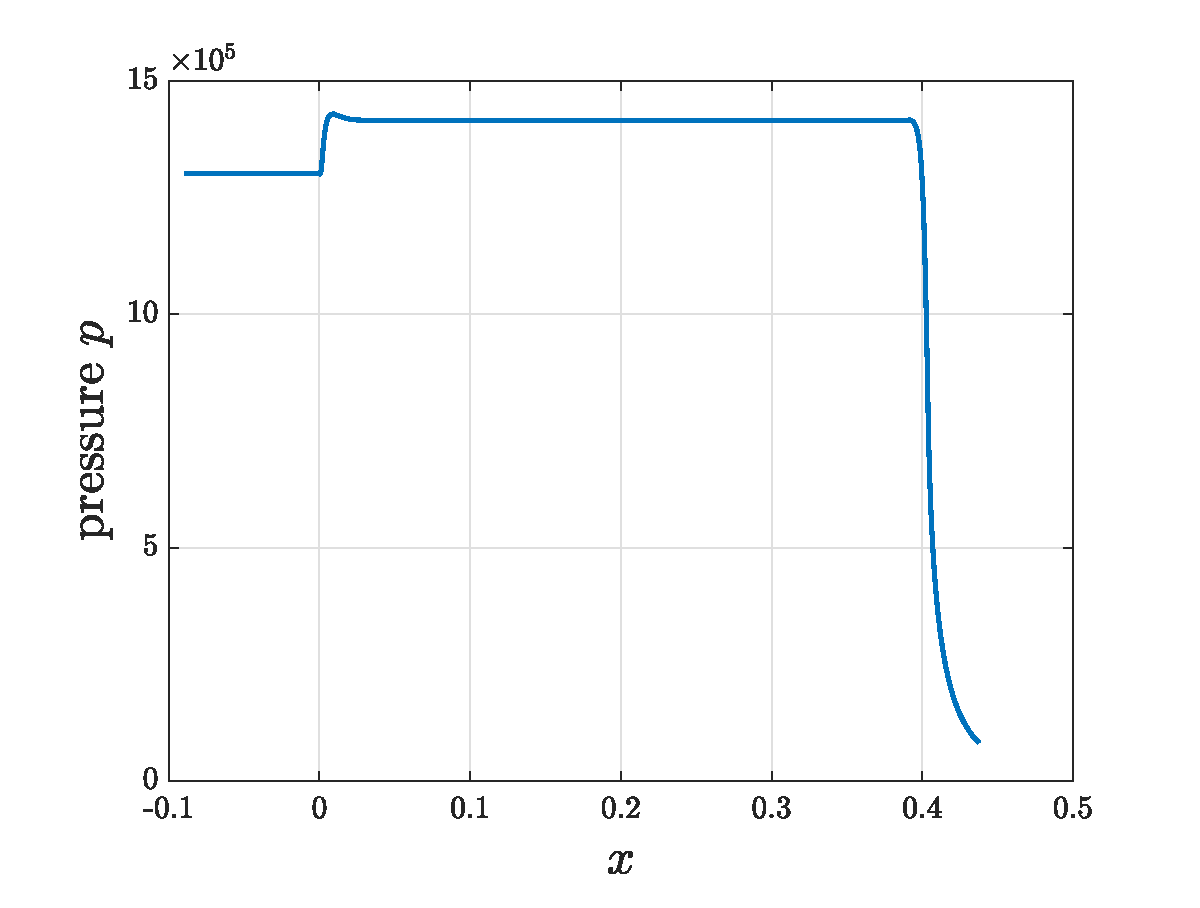
\includegraphics[width=\textwidth]{./pic/init_pressure}
%	\caption{} \label{fig:5p2.2a}
%\end{subfigure}
%\begin{subfigure}[]{0.47\linewidth}
%	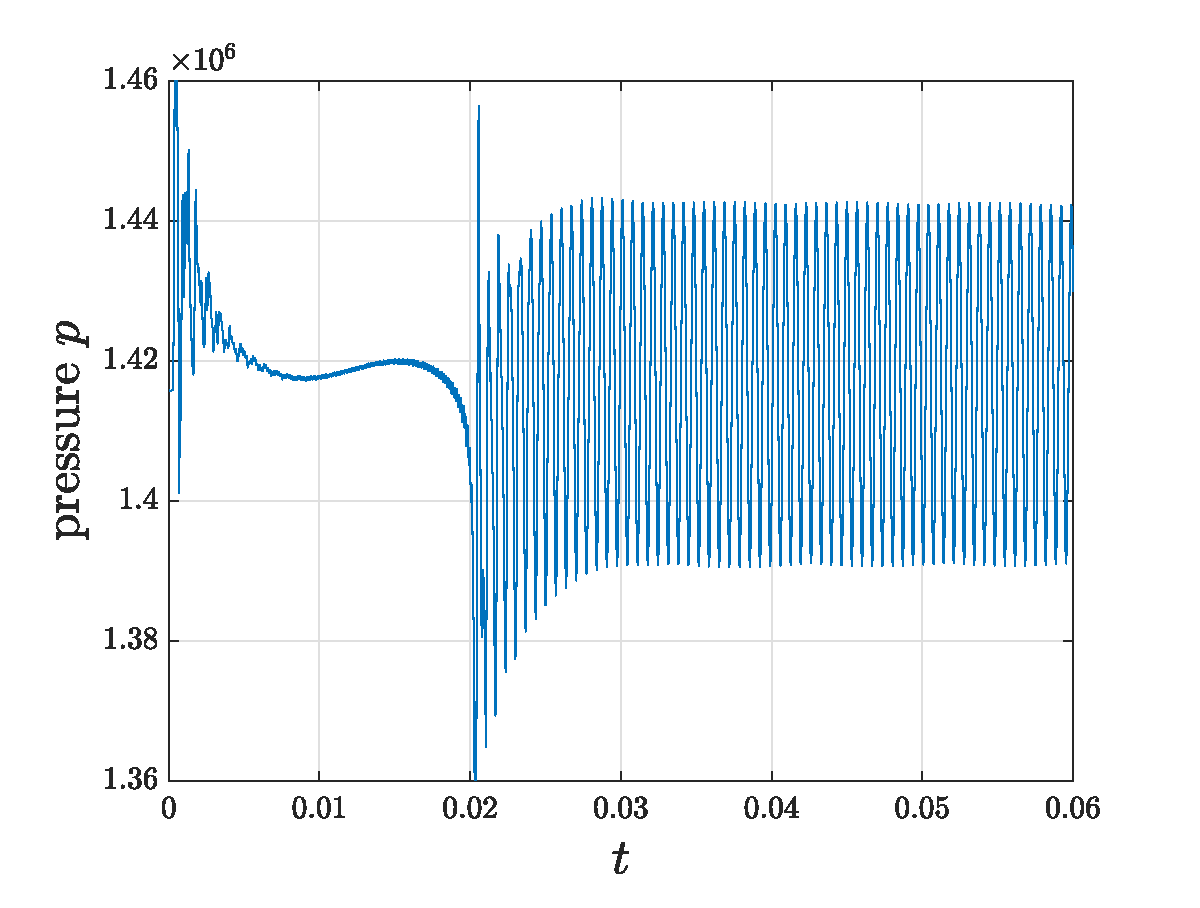
\includegraphics[width=\textwidth]{./pic/init_osc}
%	\caption{} \label{fig:5p2.2b}
%\end{subfigure} \\
%\begin{subfigure}[]{0.47\linewidth}
%	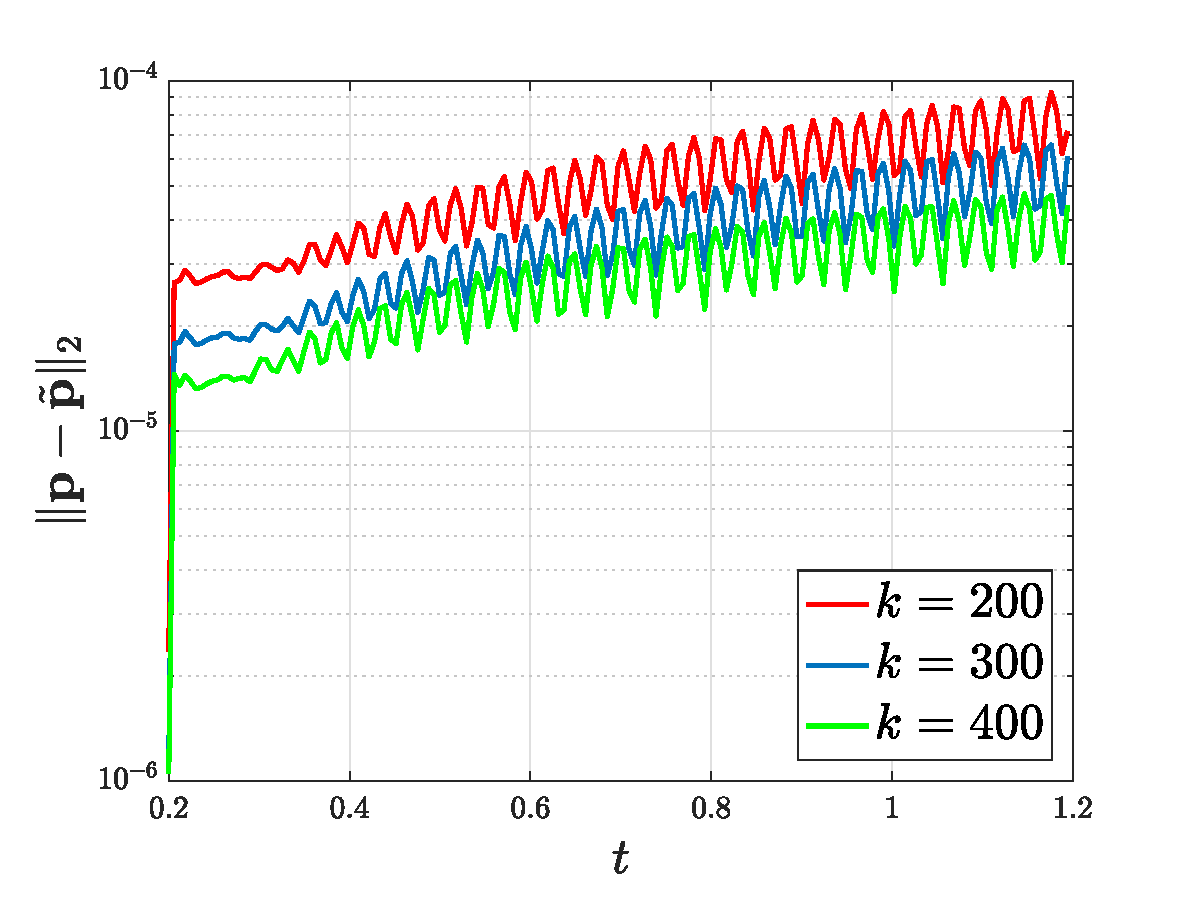
\includegraphics[width=\textwidth]{./pic/p_error}
%	\caption{} \label{fig:5p2.2c}
%\end{subfigure}
%\begin{subfigure}[]{0.47\linewidth}
%	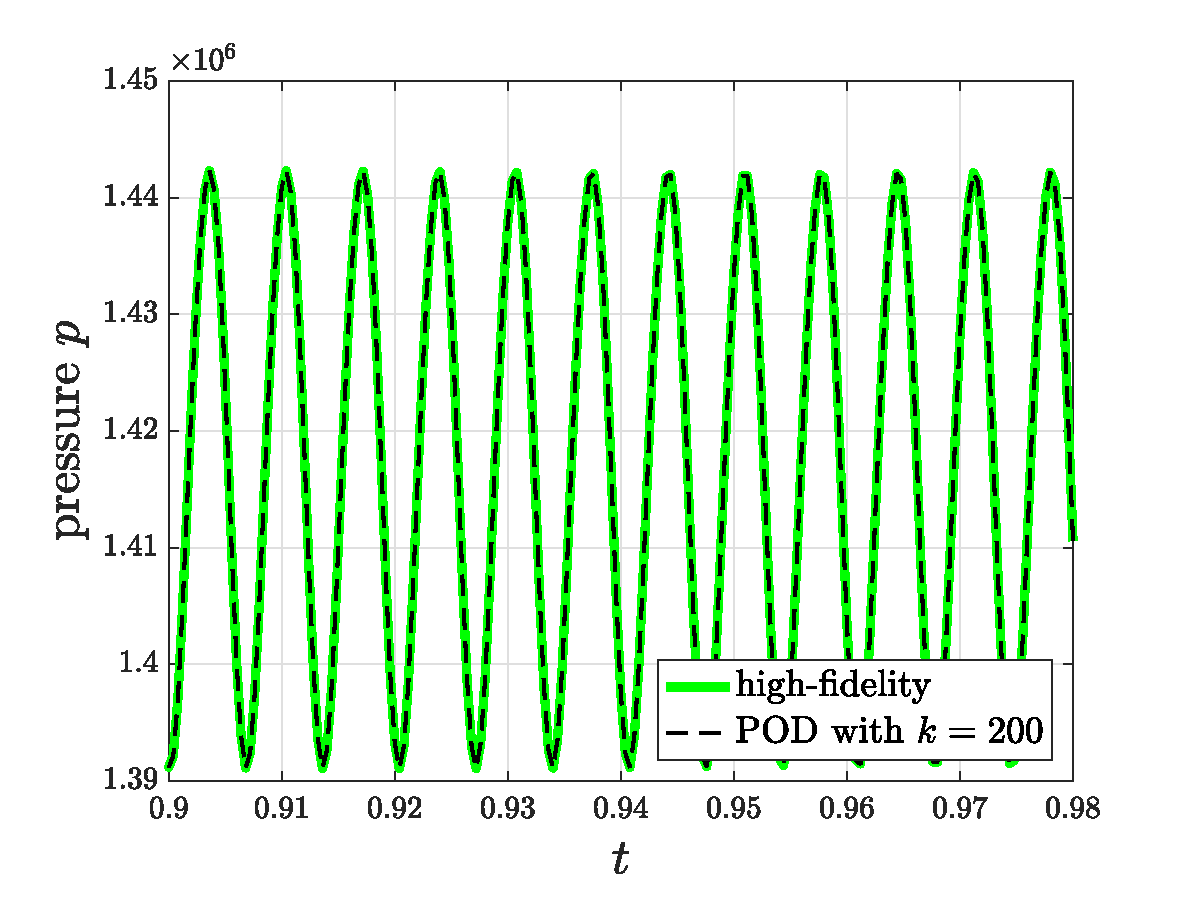
\includegraphics[width=\textwidth]{./pic/rom_freq}
%	\caption{} \label{fig:5p2.2d}
%\end{subfigure}
%\caption{(a) Pressure profile of the steady state. (b) Oscillatory mode of pressure located at $x=0.36$ for the unsteady flow. (c) Relative error between the high-fidelity and approximated pressure. (d) Approximation of the oscillations. }
%\label{fig:5p2.2}
%\end{figure}

%%%%%%%%%%%%%%%%%%%%%%%%%%%%%%%%%%%%%%%%%%%%
%%%%%%%%%%%%%%%%%%% Combustor %%%%%%%%%%%%%%%%%%%
%%%%%%%%%%%%%%%%%%%%%%%%%%%%%%%%%%%%%%%%%%%%
\begin{figure}
  \centering
  % Pressure steady
  \begin{subfigure}[]{0.48\linewidth}
  \begin{tikzpicture}[scale=0.55]
    \begin{axis}[ylabel = pressure $p$,
                 xlabel=$x$,
                 label style={font=\Large},
                 legend pos=north east,
                 %legend entries={$k=102$ Adv,$k=201$ Adv,$k=102$ Div,$k=201$ Div,$k=102$ Skew,$k=201$ Skew},
                 legend style={font=\large},
                 grid=both,
                 ticks=both,
                 width=1.4\linewidth, 
                 height=1.0\linewidth,
                 minor x tick num=1,
                 minor y tick num=2,	
                 %yticklabel style={/pgf/number format/.cd,fixed,precision=9},
                 scaled x ticks = true,
                 enlargelimits=false,
                 scale only axis,
%                 ymin=0,
                 ymax = 1500000,
                 samples = 100]
                 \addplot[color=blue,style=solid,style=ultra thick]  table[x = x, y = pressure] {./data/Combustor/pressure_steady_state.txt};
    \end{axis}%  
  \end{tikzpicture}
  \caption{}
  \label{steady_state}
  \end{subfigure}\hfill% 
  % Pressure oscilaltions
  \begin{subfigure}[]{0.48\linewidth}
  \begin{tikzpicture}[scale=0.55]
    \begin{axis}[ylabel = pressure $p$,
                 xlabel=$t$,
                 label style={font=\Large},
                 legend pos=north east,
                 %legend entries={$k=102$ Adv,$k=201$ Adv,$k=102$ Div,$k=201$ Div,$k=102$ Skew,$k=201$ Skew},
                 legend style={font=\large},
                 grid=both,
                 ticks=both,
                 width=1.4\linewidth, 
                 height=1.0\linewidth,
                 minor x tick num=1,
                 minor y tick num=2,	
                 %yticklabel style={/pgf/number format/.cd,fixed,precision=9},
                 scaled x ticks = true,
                 scaled y ticks = true,
                 enlargelimits=false,
                 scale only axis,
                 ymin=0,
%                 samples = 100,
                 xmax = 0.06,
                 ymin = 1360000,
                 ymax = 1460000,
                 tick label style={/pgf/number format/fixed} ]
                 \addplot[color=blue,style=solid,style=thick]  table[x = t, y = pressure] {./data/Combustor/ciao.txt};
    \end{axis}%  
  \end{tikzpicture}
  \caption{}
  \label{oscill_pressure}
  \end{subfigure}
  
% Total momentum
  \begin{subfigure}[]{0.48\linewidth}
  \begin{tikzpicture}[scale=0.55]
    \begin{semilogyaxis}[ylabel = $\| p-\tilde{p}\|_2$,
                 xlabel=$t$,
                 label style={font=\Large},
                 legend pos=south east,
                 legend entries={$k=200$,$k=300$,$k=300$},
                 legend style={font=\large},
                 grid=both,
                 ticks=both,
                 width=1.4\linewidth, 
                 height=1.0\linewidth,
                 minor x tick num=1,
                 minor y tick num=2,	
                 %yticklabel style={/pgf/number format/.cd,fixed,precision=9},
                 scaled x ticks = true,
                 scaled y ticks = true,
                 enlargelimits=false,
                 scale only axis,
                 samples = 300,
                 ymin = 0.000001,
                 ymax = 0.0001]
                 \addplot[color=red,style=solid,style=thick]  table[x = t, y = error] {./data/Combustor/error_200.txt};
                 \addplot[color=blue,style=solid,style=thick]  table[x = t, y = error] {./data/Combustor/error_300.txt};
                 \addplot[color=black!50!green,style=solid,style=thick]  table[x = t, y = error] {./data/Combustor/error_400.txt};
    \end{semilogyaxis}%  
  \end{tikzpicture}
  \caption{}
  \label{error_growth_comb}
  \end{subfigure}\hfill% 
  % Pressure reduction  
  \begin{subfigure}[]{0.48\linewidth}
  \begin{tikzpicture}[scale=0.55]
    \begin{axis}[ylabel = pressure $p$,
                 xlabel=$t$,
                 label style={font=\Large},
                 legend pos=north east,
                 legend entries={High fidelity,  POD with $k=200$},
                 legend style={font=\large},
                 grid=both,
                 ticks=both,
                 width=1.4\linewidth, 
                 height=1.0\linewidth,
                 minor x tick num=1,
                 minor y tick num=2,	
                 %yticklabel style={/pgf/number format/.cd,fixed,precision=9},
                 scaled x ticks = true,
                 enlargelimits=false,
                 scale only axis,
                 xmin = 0.9,
                 xmax = 0.98,
                 ymin = 1390000,
                 ymax = 1450000,
                 tick label style={/pgf/number format/fixed} ]
                 \addplot[color=green,style=solid,style=ultra thick]  table[x = t, y = pressure] {./data/Combustor/full.txt};
                 \addplot[color=black,style=dashed,style=thick]  table[x = t, y = pressure] {./data/Combustor/red.txt};
    \end{axis}%  
  \end{tikzpicture}
  \caption{}
  \label{oscill_focus}
  \end{subfigure}
  \caption{(\protect\subref{steady_state}) Pressure profile of the steady state.  (\protect\subref{oscill_pressure}) Oscillatory mode of pressure located at $x=0.36$ for the unsteady flow. (\protect\subref{error_growth_comb}) Relative error between the high-fidelity and approximated pressure. (\protect\subref{oscill_focus}) Approximation of the oscillations.} 
  \label{fig:5p2.2}
\end{figure}


The discontinuities that appear in the solution of \eqref{eq:5p2.10} suggests that a, relatively, large basis is required to resolve fine structures in the solution. In this paper, a POD basis is generated with $k=200$, $k=300$ and $k=400$ number of basis vectors. To avoid basis changes in reduced system, only one POD basis is considered for $\rho$, $\rho u$ $\rho E$ and $\rho Y_{ox}$. The explicit SSP RK3 is then used to integrated the reduced system in time, for the unsteady system. The source terms are evaluated in the high-fidelity space and then projected onto the reduced space. However, in principle, the DEIM can be applied to accelerate this evaluation. 

\Cref{error_growth_comb} shows the approximation error of the pressure, due to MOR. It is observed that the approximation is coherently enhanced as the number of basis vectors are increase. Furthermore, the approximated solution maintains high accuracy over a relatively long time-integration. The oscilations of pressure is demostrated in \Cref{oscill_focus}. It is seen that the overall behaviour of pressure is well approximated using the reduced system. Similar results are obtained for a POD basis with higher number of modes.

We note that the discrete form of \eqref{eq:5p2.10} is not in the full skew-symmetric form. Nontheless, the quisi-skew-symmetric discretization provides a remarkable stability preservation.

\section{Conclusions} \label{sec:con}

Conservation of nonlinear invariants are not, in general, guaranteed with conventional model reduction techniques. The violation of such invariants often result in a qualitatively wrong or unstable reduce system, even when the high-fidelity system is stable. This is particularly important for fluid flow, where conservation of the energy, as a nonlinear invariant of the system, is crucial for a correct numerical evaluation.

In this paper, we discuss that conservative properties of the skew-symmetric form for fluid flow can naturally be extended to the reduced system. Conventional MOR techniques preserves the skew-symmetry of differential operator which result in conservation of quadratic invariants at the level of reduced system. Furthermore, we see that the reduced system, also, contains quadratic invariants with respect to the reduced variables that approximates the invariants of the high-fidelity system. This results in construction of a physically meaningful reduced system, rather than a mere couple systems of differential equations.

Numerical experiments of the incompressible and compressible Euler equation confirms conservation of mass, momentum and energy for the model reduction with the skew-symmetric discretization. It is seen that when a non-skew-symmetric form, e.g. divergence form or advective form, is considered, MOR does not necessarily yield a stable reduced system. On the other hand the skew-symmetric form consistently yields a robust reduced system over long time-integration, even if when the reduce space does not represent the high-fidelity solution accurately. 

Finally, a MOR of a quasi-skew-symmetric form for the CVRC model is presented. Although this model is not in a full skew-symmetric form and am explicit Runge-Kutta method used for time-integration, we still recover remarkable stability preservation. 


\bibliographystyle{plain}
\bibliography{references}

\end{document}
